\documentclass{chapters/_template-uc2} 

\department{Department of Fundamental Computing and its Applications(IFA)}
\specialty{Data Sciences and Artificial Intelligence (SDIA)}
\title{Intelligent Polypectomy: A Reinforcement Learning Approach for Polyp Removal} 
\studentFullnameA{Hamdi Ramdane}
\studentFullnameB{Fellah Haithem}
\supervisorFullnameA{Pr. Chaker Mezioud}
\session{June 2026}

%% Preamble - imports and configurations
%-------------------------------------------------------
% Preamble - All imports and configurations
%-------------------------------------------------------

% Additional packages (subcaption, booktabs, float are loaded by the class file)

%-------------------------------------------------------
% Figure placement - keep figures close to their text
%-------------------------------------------------------
\renewcommand{\topfraction}{0.9}
\renewcommand{\bottomfraction}{0.9}
\renewcommand{\textfraction}{0.1}
\renewcommand{\floatpagefraction}{0.7}
\setcounter{topnumber}{3}
\setcounter{bottomnumber}{3}
\setcounter{totalnumber}{5}

%-------------------------------------------------------
% Graphics path
%-------------------------------------------------------
\graphicspath{{assets/}}

%-------------------------------------------------------
% Listings (Source codes) configuration
%-------------------------------------------------------
\definecolor{color-lst-string}{RGB}{166,95,18}
\definecolor{color-lst-annotation}{RGB}{128,128,0}
\definecolor{color-lst-constant}{RGB}{5,133,5}
\definecolor{color-lst-keyword}{RGB}{33,33,255}
\definecolor{color-lst-class}{RGB}{0,112,192}
\definecolor{color-lst-accessor}{RGB}{125,0,84}
\definecolor{color-lst-comment}{RGB}{168,166,171}

% Python language definition
\lstdefinelanguage{Python}{
	morekeywords={import,from,class,def,for,while,if,else,elif,return,try,except,with,as,lambda,None,True,False,and,or,not,in,is},
	sensitive=true,
	morecomment=[l]{\#},
	morestring=[b]',
	morestring=[b]",
}


\begin{document}

\frontmatter
	\maketitlepage
	\pagestyle{plain}
	\chapter*{Acknowledgments}
\addcontentsline{toc}{chapter}{Acknowledgments}

This secion is commented out will be revealed later.
% Huge thanks to \textbf{\studentFullnameB} for the way the project kept moving through
% people, not just code. Networking skills helped reach the right sources quickly, find
% answers at the right time, and unblock practical issues that could have easily cost
% weeks. Equally important was the patience with the AI side of the work: unstable
% experiments, training runs failing for non-obvious reasons, results needing multiple
% iterations, and long debugging sessions. Consistent effort on reruns, checks, and model
% improvement helped push the output to a level that could be explained and defended.

% Massive thanks to \textbf{\studentFullnameA} for speed and precision when deadlines
% were close. Fast delivery did not replace quality: sharp results helped turn scattered
% ideas into concrete sections, clear figures, and coherent decisions. Strong
% prioritization kept the work focused, and clean deliverables (writing, formatting, and
% iteration on drafts) kept the manuscript consistent from start to finish.

% Special thanks to \textbf{\supervisorFullnameA} for choosing us for this work, for the
% trust placed in the team from the start, and for guidance that kept the scope realistic.
% Clear feedback and high standards helped shape this work into something that can be
% presented and defended with confidence.
	\input{chapters/002_dedicate}
	%% =============================================================================
%% ABSTRACT (English + French + Arabic)
%% =============================================================================

\clearpage
\phantomsection
\addcontentsline{toc}{chapter}{Abstract}

\begin{center}
\textbf{\Large Abstract}
\end{center}
\vspace{0.2cm}
\indent Colorectal cancer is a massive global problem, causing roughly 10\% of all cancer cases. The most effective intervention is the early detection and resection of suspicious polyps. However, navigating the 2,000 cm\textsuperscript{2} surface area of the colon with a flexible endoscope presents a significant technical challenge. It generally requires two coordinated physicians, relying on rapid decision-making and steady motor control under pressure. Rather than relying on costly robotic hardware, we pursued a software-centric approach. We developed a semi-autonomous agent to manage the core navigation tasks within a high-fidelity virtual colon. To manage complexity, we divided the challenge: one agent steers the endoscope tip through the colonic lumen, and once a polyp is identified, a second agent takes over to accurately position a wire snare around it. Both utilize Deep Reinforcement Learning with Proximal Policy Optimization (PPO), Convolutional Neural Networks (CNN), and a Long Short-Term Memory (LSTM) core for spatial awareness. Consequently, polypectomy extends beyond basic image recognition; it is a highly complex, sequential decision-making problem. By structuring the reward system to incentivize safe maneuvers and penalize collisions, the agents learned to balance the preservation of healthy tissue with the execution of precise resections. Our unique dual-sphere proxy proved that these vision-only agents can navigate and capture polyps under realistic, noisy conditions.

\vspace{0.5cm}
\noindent\textbf{Keywords:} colorectal cancer, deep reinforcement learning, PPO, CNN, virtual simulation, polypectomy, snare capture

\clearpage
\begin{center}
\textbf{\Large R\'esum\'e}
\end{center}
\vspace{0.2cm}
\indent Le cancer colorectal cause environ 10 \% des cas de cancer mondiaux. La meilleure solution reste la détection et la résection précoce des polypes. Cependant, naviguer dans un côlon de 2 000 cm\textsuperscript{2} avec un endoscope délicat est un défi technique majeur. Cette procédure nécessite généralement deux médecins coordonnés, reposant sur leur précision et rapidité sous une pression intense. Plutôt que de développer des robots coûteux, nous avons privilégié une approche logicielle. Nous avons créé un agent semi-autonome pour accomplir le gros du travail dans un environnement virtuel hyper-réaliste. Pour gérer la complexité, nous avons divisé le défi : un agent dirige l'embout de l'endoscope à travers les tunnels roses (côlon), et une fois un polype repéré, un deuxième agent prend le relais pour refermer délicatement une anse métallique autour de lui. Les deux utilisent l'Apprentissage par Renforcement Profond avec Proximal Policy Optimization (PPO), des Réseaux de Neurones Convolutifs (CNN) et une mémoire Long Short-Term Memory (LSTM) pour ne pas se perdre. La polypectomie s'avère être un problème décisionnel séquentiel complexe. En entraînant nos agents par renforcement, ils ont appris à équilibrer la précision de la coupe avec la préservation des tissus sains. Notre modèle montre que des agents basés uniquement sur la vision peuvent naviguer et réussir des interventions sous des conditions de bruit réalistes.

\vspace{0.5cm}
\noindent\textbf{Mots-cl\'es:} cancer colorectal, apprentissage par renforcement profond, PPO, CNN, simulation virtuelle, polypectomie, capture par anse

\clearpage
\begin{Arabic}
\begin{center}
\textbf{\Large ملخص}
\end{center}
\vspace{0.2cm}
\indent يُعد سرطان القولون والمستقيم صداعاً عالمياً هائلاً، حيث يتسبب في حوالي \textenglish{10\%} من جميع حالات السرطان. أفضل حل؟ اكتشاف الأورام الحميدة المشبوهة وقطعها مبكراً. لكن توجيه منظار دقيق داخل قولون بمساحة \textenglish{2000} سم\textsuperscript{2} أمر بالغ الصعوبة! يتطلب الأمر عادةً طبيبين منسقين، حيث يعتمد كلياً على قراراتهما السريعة وأيديهما الثابتة تحت ضغط شديد. بدلاً من بناء روبوتات باهظة الثمن، اتخذنا نهجاً برمجياً جريئاً! قمنا بإنشاء وكيل شبه مستقل للقيام بالعمل الشاق داخل قولون افتراضي فائق الواقعية. ولإبقاء الأمور تحت السيطرة، قمنا بتقسيم التحدي: حيث يقوم الوكيل الأول بتوجيه طرف المنظار عبر الأنفاق الوردية (القولون)، وبمجرد اكتشاف ورم، يتولى وكيل ثانٍ مهمة إغلاق حلقة سلكية برفق حوله. كلاهما يستخدم التعلم المعزز العميق (\textenglish{PPO}) والشبكات العصبية التلافيفية (\textenglish{CNN}) مع ذاكرة (\textenglish{LSTM}) حتى لا يضيعا. اتضح أن استئصال السليلة ليس مجرد تعرف أساسي على الصور؛ بل هو لعبة قرارات متسلسلة في غاية التعقيد! من خلال إعطاء الذكاء الاصطناعي الخاص بنا مكافآت على الحركات الجيدة وعقوبات عند الاصطدام، تعلموا الموازنة بشكل مثالي بين الحفاظ على الأنسجة السليمة وإجراء عمليات قطع دقيقة. أثبت نظام الوكيل مزدوج الكرات الفريد لدينا أن هؤلاء الوكلاء المعتمدين على الرؤية فقط يمكنهم التنقل والتقاط الأورام الحميدة في ظل ظروف واقعية صاخبة.

\vspace{0.5cm}
\noindent\textbf{الكلمات المفتاحية:} سرطان القولون والمستقيم، التعلم المعزز العميق، \textenglish{PPO}، \textenglish{CNN}، محاكاة افتراضية، استئصال السليلة، الالتقاط بالحلقة السلكية.
\end{Arabic}

\clearpage
	\tableofcontents
	\listoffigures
	\listoftables

\mainmatter
	\pagestyle{fancy}
	\chapter*{General Introduction}
\addcontentsline{toc}{chapter}{General Introduction}
\chaptermark{General Introduction}
\label{chap:general_introduction}

\section*{Project Background}
\addcontentsline{toc}{section}{Project Background}

Colorectal cancer is still a major public health problem worldwide \cite{sung2021globocan}.
One of the best ways to reduce that risk is to remove suspicious polyps early, which is
why \textbf{polypectomy} matters so much \cite{winawer1993polypectomy}. Even though the
procedure is common, it is not simple: the final result depends on the operator, the
quality of the view, the shape of the lesion, and the pressure of making good decisions
in real time.

Even with good screening programs, tandem colonoscopy studies still report meaningful
\textbf{adenoma} (a type of polyp that can become cancerous) miss rates
\cite{zhao2019adenomaMiss}. Also, quality measures like \textbf{adenoma detection rate}
are linked with future colorectal cancer risk \cite{corley2014adr}.

This work studies how intelligent methods can support \textbf{polypectomy} by
combining computer vision and \textbf{reinforcement learning} (RL, learning by trial and
error using rewards). The main idea is to help an agent read the scene, understand what
is happening, and choose better actions in a simulated setting. The goal here is to
study how perception and action work together in a sequence of decisions, not to build a
clinical detector.

\section*{Problem}
\addcontentsline{toc}{section}{Problem}
\vspace{-0.5em}
The core problem is to design a \textbf{learning-based control and perception framework}
for \textbf{polypectomy-like tasks} that works under realistic constraints:
\textbf{partial and noisy visual observations}, \textbf{delayed or limited instrument control},
and strict \textbf{safety requirements}. Concretely, the main technical challenges are to:
interpret noisy imagery reliably, decide actions that avoid tissue damage, time interventions
under uncertainty, and remain robust when the visual scene changes or tools occlude
important features.

Concretely, this work addresses the following specific questions:
\begin{itemize}
\item \textbf{Perception → Action:} How can an agent learn to use visual observations
	(single frames, short temporal stacks, or depth cues) to select \textbf{safe and effective}
	actions during a polypectomy-like task?
\item \textbf{Learning & Transfer:} How can training be organised so the model improves
	in \textbf{simulation} while enforcing \textbf{safety limits} and conservative procedures
	for later transfer to real hardware?
\item \textbf{Reward & Representation:} How should the \textbf{reward function} and
	\textbf{observation encoding} be designed so the agent balances \textbf{tissue preservation},
	precision of resection, and task efficiency?
\item \textbf{Robustness:} How to make policies resilient to \textbf{domain shift} such as
	camera viewpoint changes, lighting variability, specular highlights, and instrument occlusion?
\item \textbf{Safety Mechanisms:} What \textbf{safety checks}, motion limits, and fallback
	strategies are required to prevent harmful actions during transfer from simulation to
	a physical endoscope?
\item \textbf{Evaluation:} Beyond simple success/failure, which metrics (\textbf{stability},
	\textbf{precision}, \textbf{efficiency}, and \textbf{clinician acceptability}) best capture
	practical usefulness?
\end{itemize}

This problem is motivated by the project theme: build a \textbf{learning-based system}
for sequential decision-making in \textbf{simulated polypectomy tasks}. The aim is to
explore technical solutions that prioritise safety, interpretability, and robust
behaviour under realistic visual and control constraints.

\section*{Objectives}
\addcontentsline{toc}{section}{Objectives}
The objectives of this work are:
\begin{itemize}
\item to review the clinical and technical background of \textbf{polypectomy} and the main
intelligent methods linked to it;
\item to study how machine learning, deep learning, and \textbf{reinforcement learning}
can help medical decision-making;
\item to design a learning-based framework that fits sequential decision-making in
polyp removal;
\item to identify the evaluation criteria that matter most for performance, stability,
and practical usefulness.
\end{itemize}

\section*{Proposed Approach}
\addcontentsline{toc}{section}{Proposed Approach}
In this work, we propose a learning-based framework that combines simple visual
processing with sequential decision learning. The main objectives are to build a safe
simulation environment, train agents that can act reliably in that environment, and
evaluate how well learned policies generalize across cases.

Main solutions and steps:
\begin{itemize}
\item \textbf{Simulation and data:} build a Unity-based simulated environment with
predefined targets and controls for the endoscope and tools.
\item \textbf{Learning pipeline:} use convolutional networks (CNNs) for visual encoding
and reinforcement learning (PPO) for sequential control, with careful reward shaping.
\item \textbf{Safety and limits:} design safety checks, motion limits, and conservative
transfer steps for any prototype testing.
\item \textbf{Evaluation:} define clear metrics (success rate, stability, efficiency) and
compare learned behavior to baseline scripted or expert demonstrations.
\end{itemize}

These solutions target the problem by combining perception, action, and safe practice
within a controlled simulation.

\section*{Document Plan}
\addcontentsline{toc}{section}{Document Plan}
The document is arranged in two main parts that follow from the repository's scope:

\begin{itemize}
\item \textbf{Chapter 1 --- State of the Art:} a concise review that situates the
	clinical problem (colorectal cancer and polypectomy), summarises key clinical
	metrics and risks, and surveys technical approaches from computer vision and
	reinforcement learning that are relevant to the project. This chapter highlights
	practical gaps and limitations in current methods that motivate the system design.

\item \textbf{Chapter 2 --- Contributions:} an account of the implemented system and
	the original contributions. In short, this chapter presents an attempt on a
		extbf{two-phase endoscope reinforcement learning system} that combines a
		extbf{simulation environment}, a \textbf{perception module} (visual encoder / CNN),
	and a \textbf{two-level control strategy} (coarse navigation + fine manipulation)
	trained with reinforcement learning. The chapter documents the design choices,
	safety measures, training setup, and evaluation metrics used to assess stability,
	precision, and practical usefulness.
\end{itemize}

Overall, the document first establishes the clinical and technical context, then
presents the contributions and the implemented two-phase system together with its
empirical evaluation.
	\chapter{State of the Art}
\label{chap:state_of_the_art}

\section*{Introduction}
\addcontentsline{toc}{section}{Introduction}
This chapter brings together the clinical and technical background that supports the
work. The basic idea is simple: if we want to build a useful endoscope agent, we have
to understand the medical workflow, the \textbf{vision methods} that read the scene, and the
\textbf{learning methods} that decide what to do next.

In this context, clinical guidance on \textbf{colorectal polypectomy} and endoscopic resection
gives us the safety baseline \cite{ferlitsch2017esge,kaltenbach2020usmstf}. At the same
time, recent clinical trials show that real-time computer-aided detection can improve
lesion detection during routine colonoscopy \cite{wang2019cade,repici2020cade}.

The chapter moves from the clinical context to the learning methods used in intelligent
systems. Along the way, we keep an eye on the practical things that matter most here:
\textbf{data quality}, \textbf{safety}, \textbf{robustness}, and \textbf{evaluation}. Those are not just side details; they
shape the design choices in the rest of the document.

\textbf{Chapter roadmap.} We start with colorectal polyps and polypectomy, then move to
Artificial Intelligence as the broader field. After that, we cover reinforcement learning
as the main framework for sequential decision-making, and we review the neural
architectures used for perception and temporal modeling (\textbf{CNN} and \textbf{LSTM}). We end with
Proximal Policy Optimization (\textbf{PPO}), the policy-gradient method used in the simulation.
\clearpage
\section{Endoscopic Polypectomy and Colorectal Polyps}
\label{sec:polypectomy}
\subsection{What is a Polyp?}
A \textbf{colorectal polyp} is an abnormal growth from the lining of the colon or rectum. It can be small and flat or larger and on a stalk. The most common precancerous type is called an \textbf{adenoma}, which is a glandular polyp with a higher risk of becoming cancer over time, so it is often removed during colonoscopy even when it does not yet cause symptoms.

This is why polyp size, shape, and appearance matter in practice: the endoscopist has to decide quickly whether the lesion should be removed and how much risk is involved.


\begin{figure}[H]
\centering
\setlength{\fboxsep}{4pt}% padding for frame
\fbox{%
	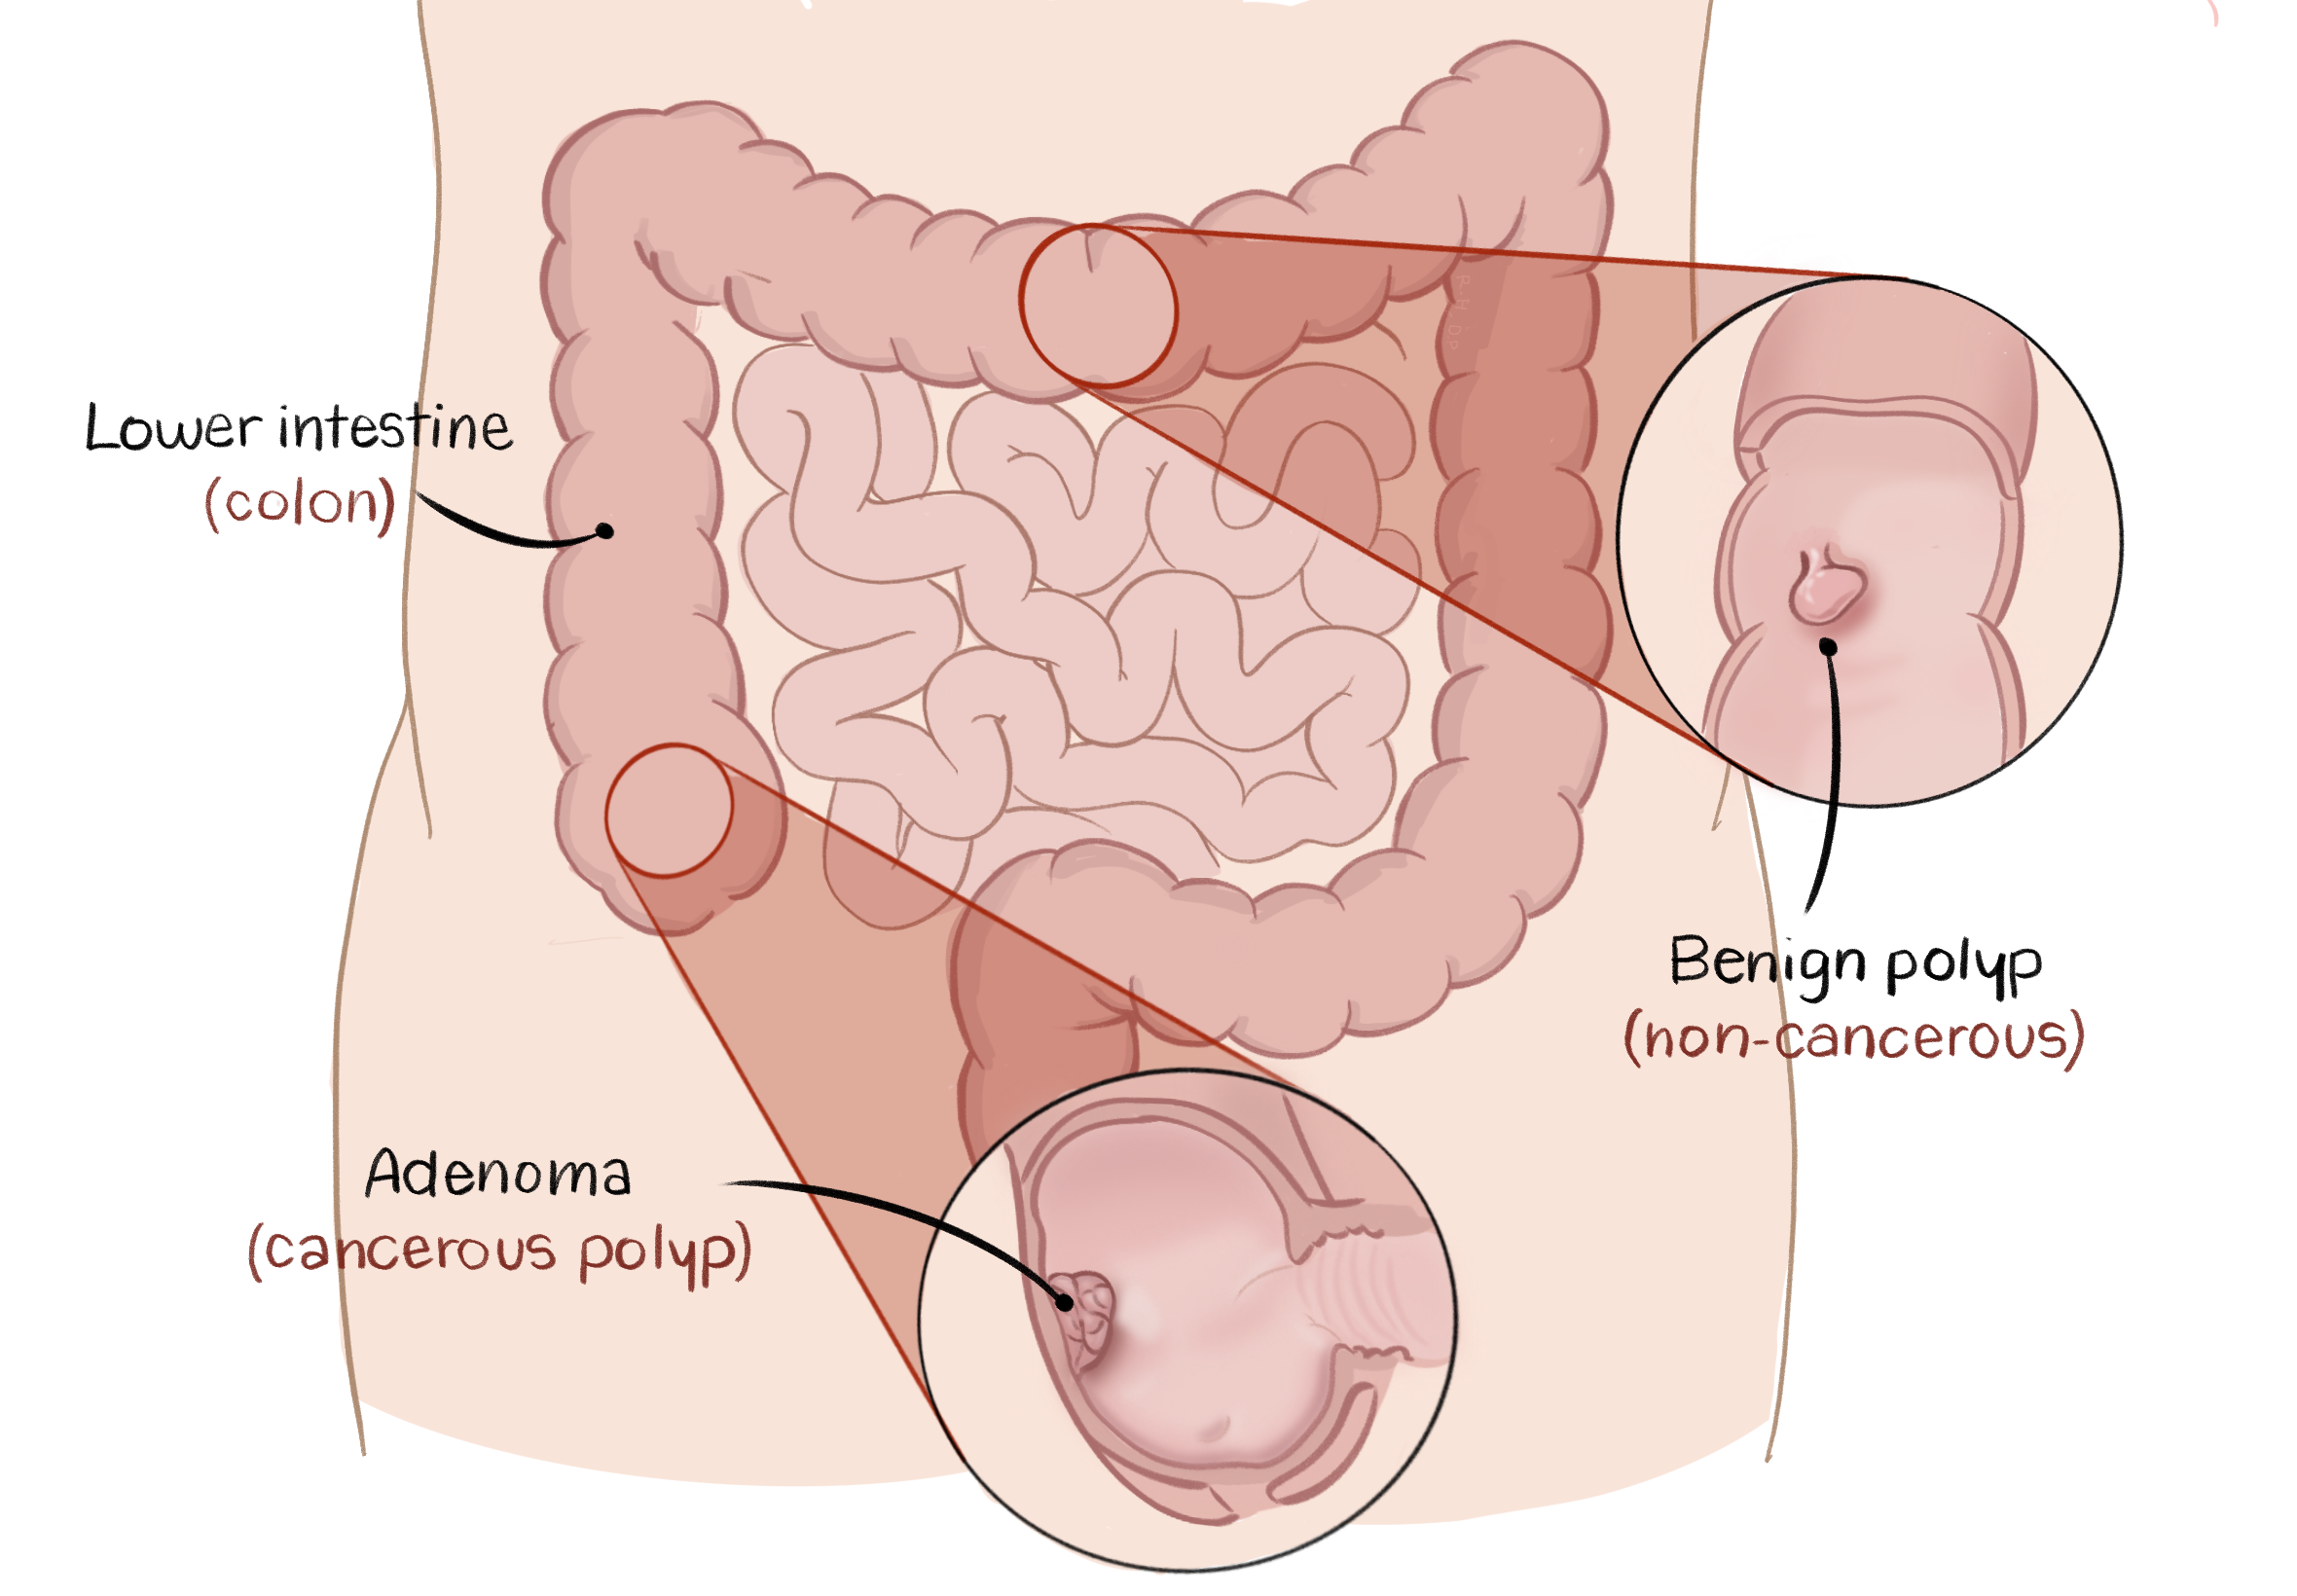
\includegraphics[width=1\linewidth,trim=0cm 0cm 1cm 0cm,clip]{assets/illustration-colon-polyps.png}%
}
\caption{Illustration of polyps inside the colon.}
\label{fig:colon_polyps}
\end{figure}

After removal, polyps are sent for \textbf{histology} to check for cancer or high‑risk features. \textbf{Small polyps} are often removed during the same colonoscopy, while larger or complex lesions may need \textbf{advanced techniques} or referral. The choice balances \textbf{completeness} of removal and patient \textbf{safety}.

\begin{figure}[H]
\centering
\setlength{\fboxsep}{4pt}% padding for frame
\fbox{%
	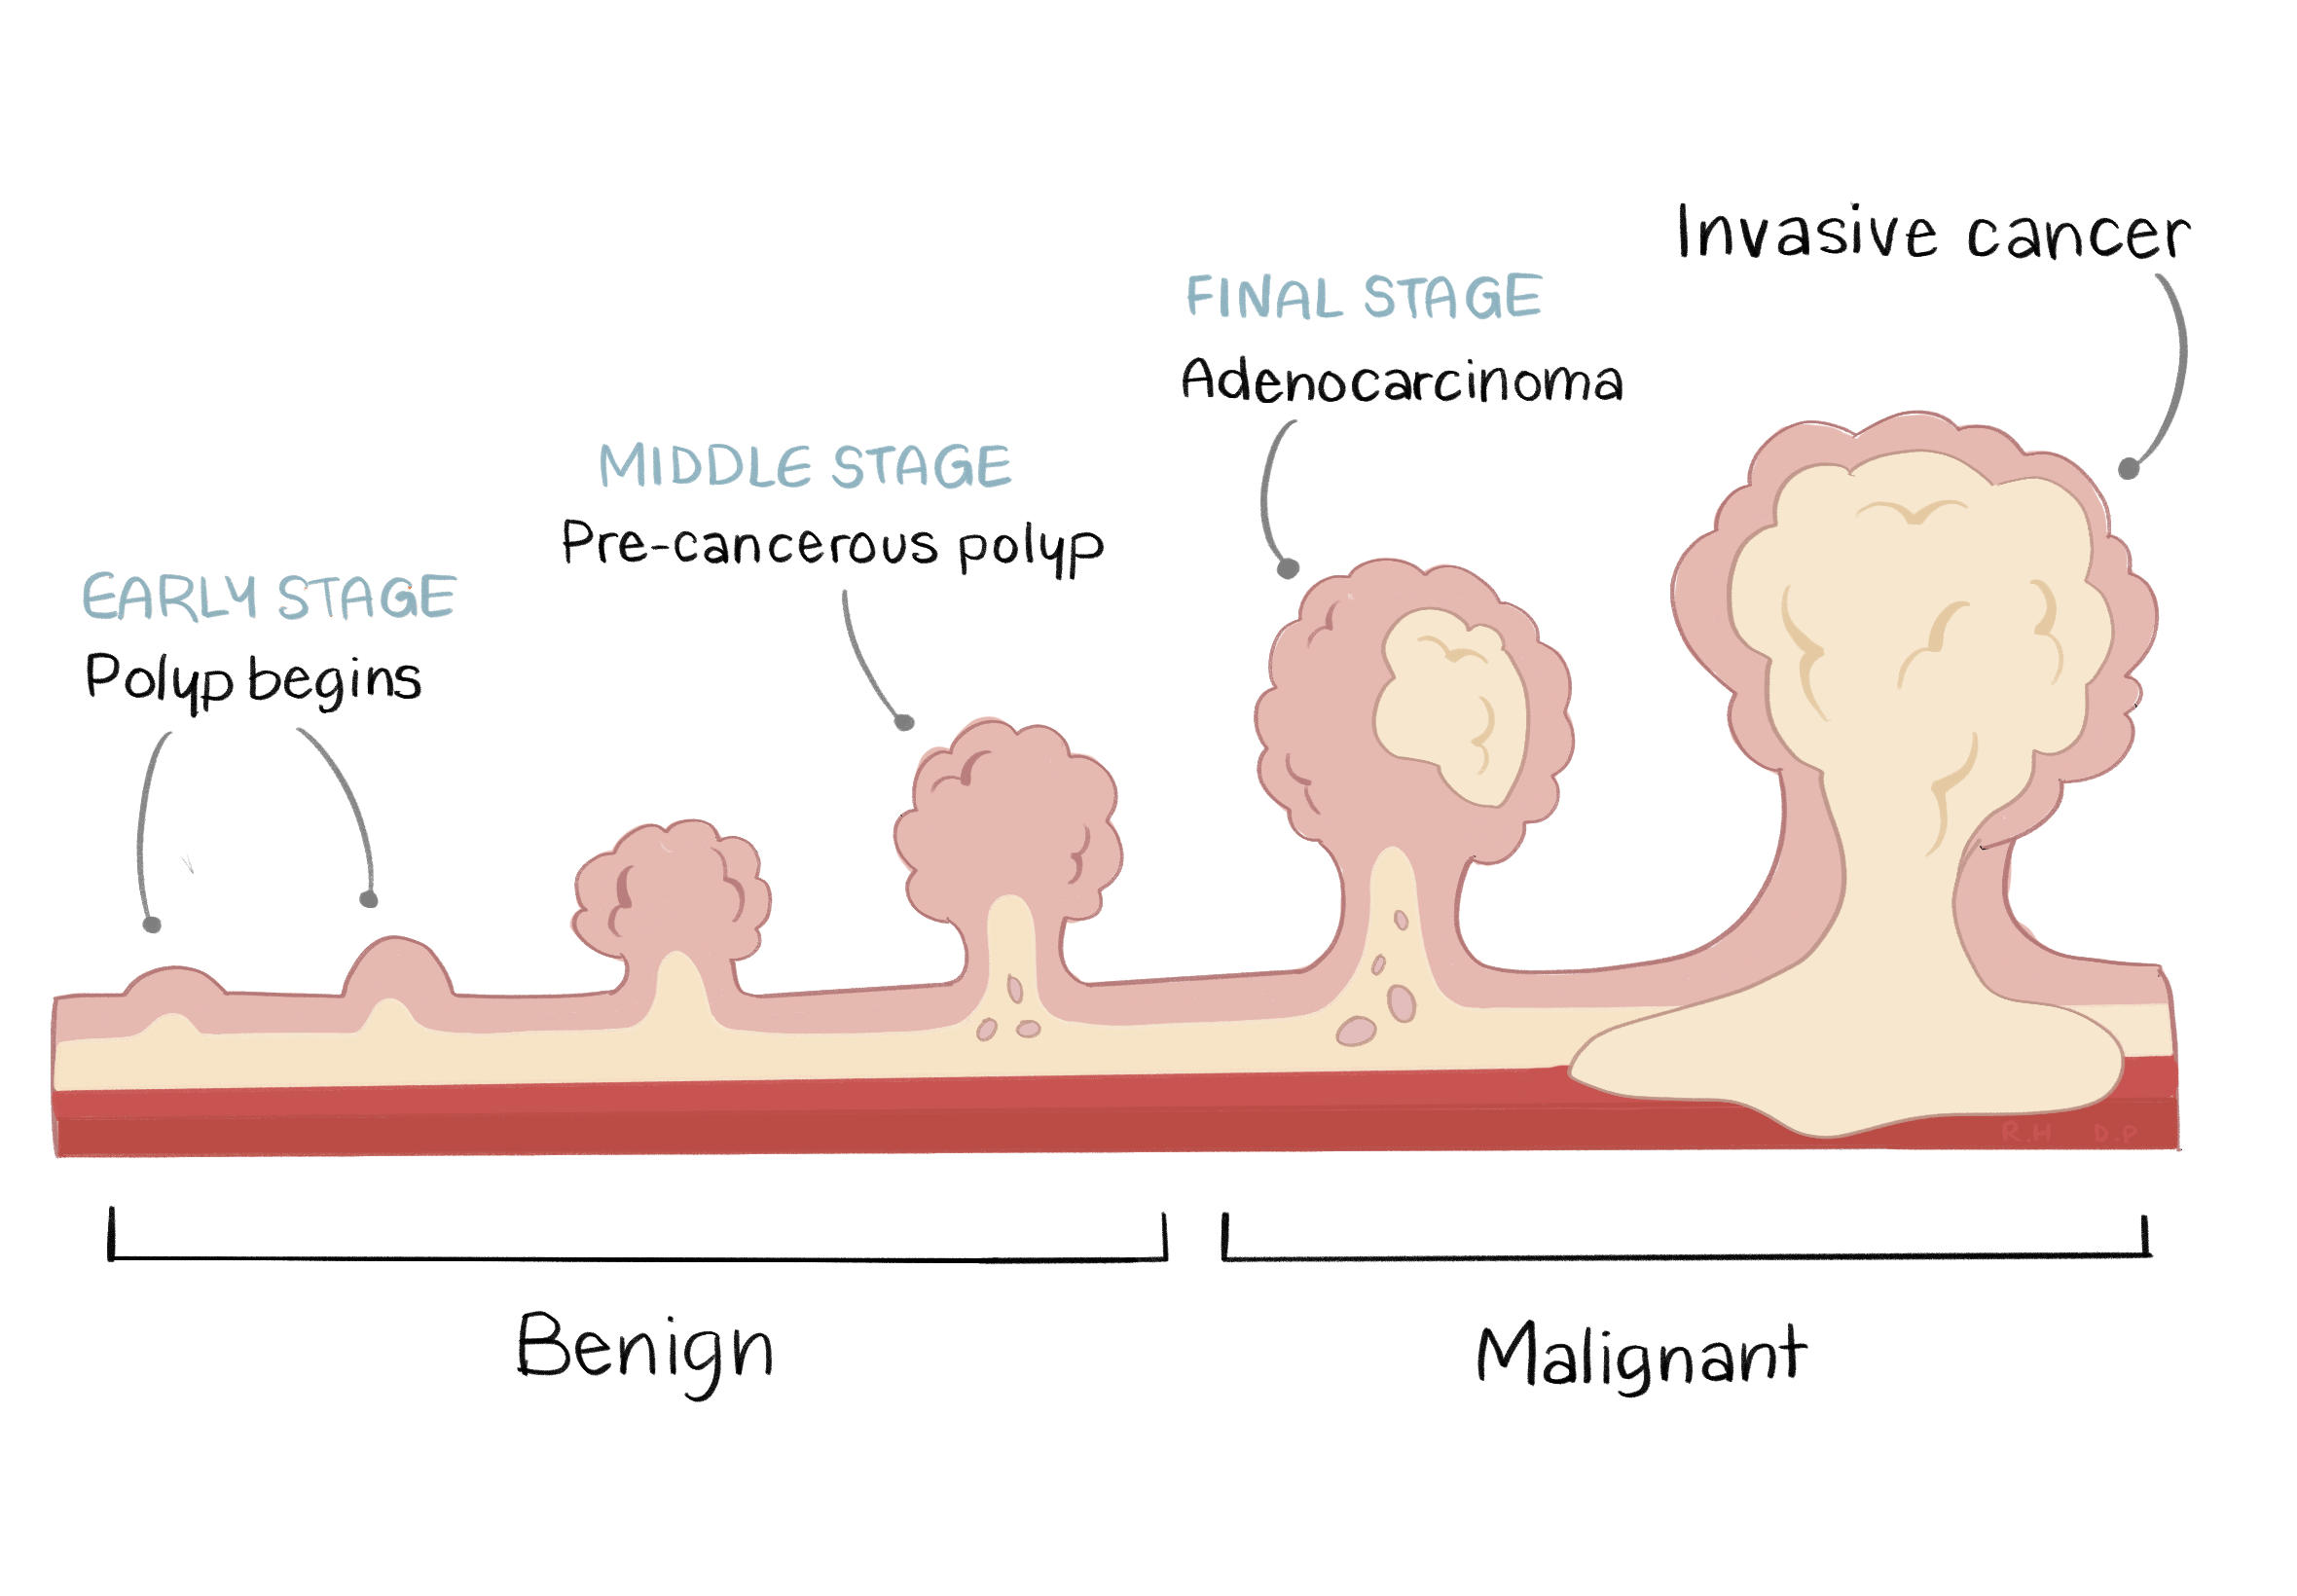
\includegraphics[width=1\linewidth,trim=1cm 6cm 2cm 4cm,clip]{assets/illustration-polyp-growth.png}%
}
\caption{Illustration of a colorectal polyp (growth stages).}
\label{fig:colorectal_polyp}
\end{figure}

Colorectal polyps are very common. Studies show that about \textbf{25--30\,\%} of adults over 50 have at least one adenomatous polyp, and this number goes up to \textbf{40--50\,\%} by age 70 \cite{strum2016prevalence}. Most polyps are small, usually under \textbf{10\,mm}, and they do not cause any symptoms. However, a small number of them follow the \textbf{adenoma to carcinoma sequence}, which is a step-by-step process where normal tissue slowly turns into cancer over \textbf{10--15 years} \cite{leslie2024polyps}. Because this process takes so long, screening is very useful since it gives doctors a wide window to find and remove polyps before they become dangerous.

The effect of removing polyps is significant. The well-known \textbf{National Polyp Study} showed that polypectomy during colonoscopy can reduce the chance of getting colorectal cancer by \textbf{76--90\,\%} \cite{winawer1993polypectomy}. Other research found that for every \textbf{1\,\%} increase in a doctor's \textbf{adenoma detection rate} (ADR), there is a \textbf{3\,\%} drop in the risk of colorectal cancer appearing later \cite{corley2014adr}. Because of this, the ADR is now used as a quality measure, and guidelines say it should be at least \textbf{25\,\%} \cite{lieberman2014screening}. Even so, studies estimate that around \textbf{26\,\%} of adenomas are still \textit{missed} during a normal examination, especially flat and right-sided ones \cite{zhao2019adenomaMiss}.

Looking at the bigger picture, colorectal cancer is the \textbf{third most common} cancer in the world and the \textbf{second leading} cause of cancer death. In 2022 alone, there were about \textbf{1.9 million} new cases and \textbf{900\,000} deaths \cite{iarc2024globocan,sung2021globocan}. These numbers show why organised screening programmes are so important. In countries like the UK, Germany, and parts of the US where screening is well established, polypectomy has helped reduce colorectal cancer deaths over time.

\clearpage
\subsection{What is an Endoscope?}
An \textbf{endoscope} is a long, flexible tube with a tiny camera and a light at the tip. Doctors use it to look inside the body without making any cuts. During a colonoscopy, the endoscope goes in through the rectum and moves along the colon so the doctor can check the inner lining for anything unusual, like polyps. It also has small channels inside that let the doctor pass tools such as snares or forceps to take samples or remove lesions. Controlling the scope, the camera angle, and the tools all at the same time is quite difficult and needs a lot of practice.

\begin{figure}[H]
\centering
\setlength{\fboxsep}{4pt}
\fbox{%
	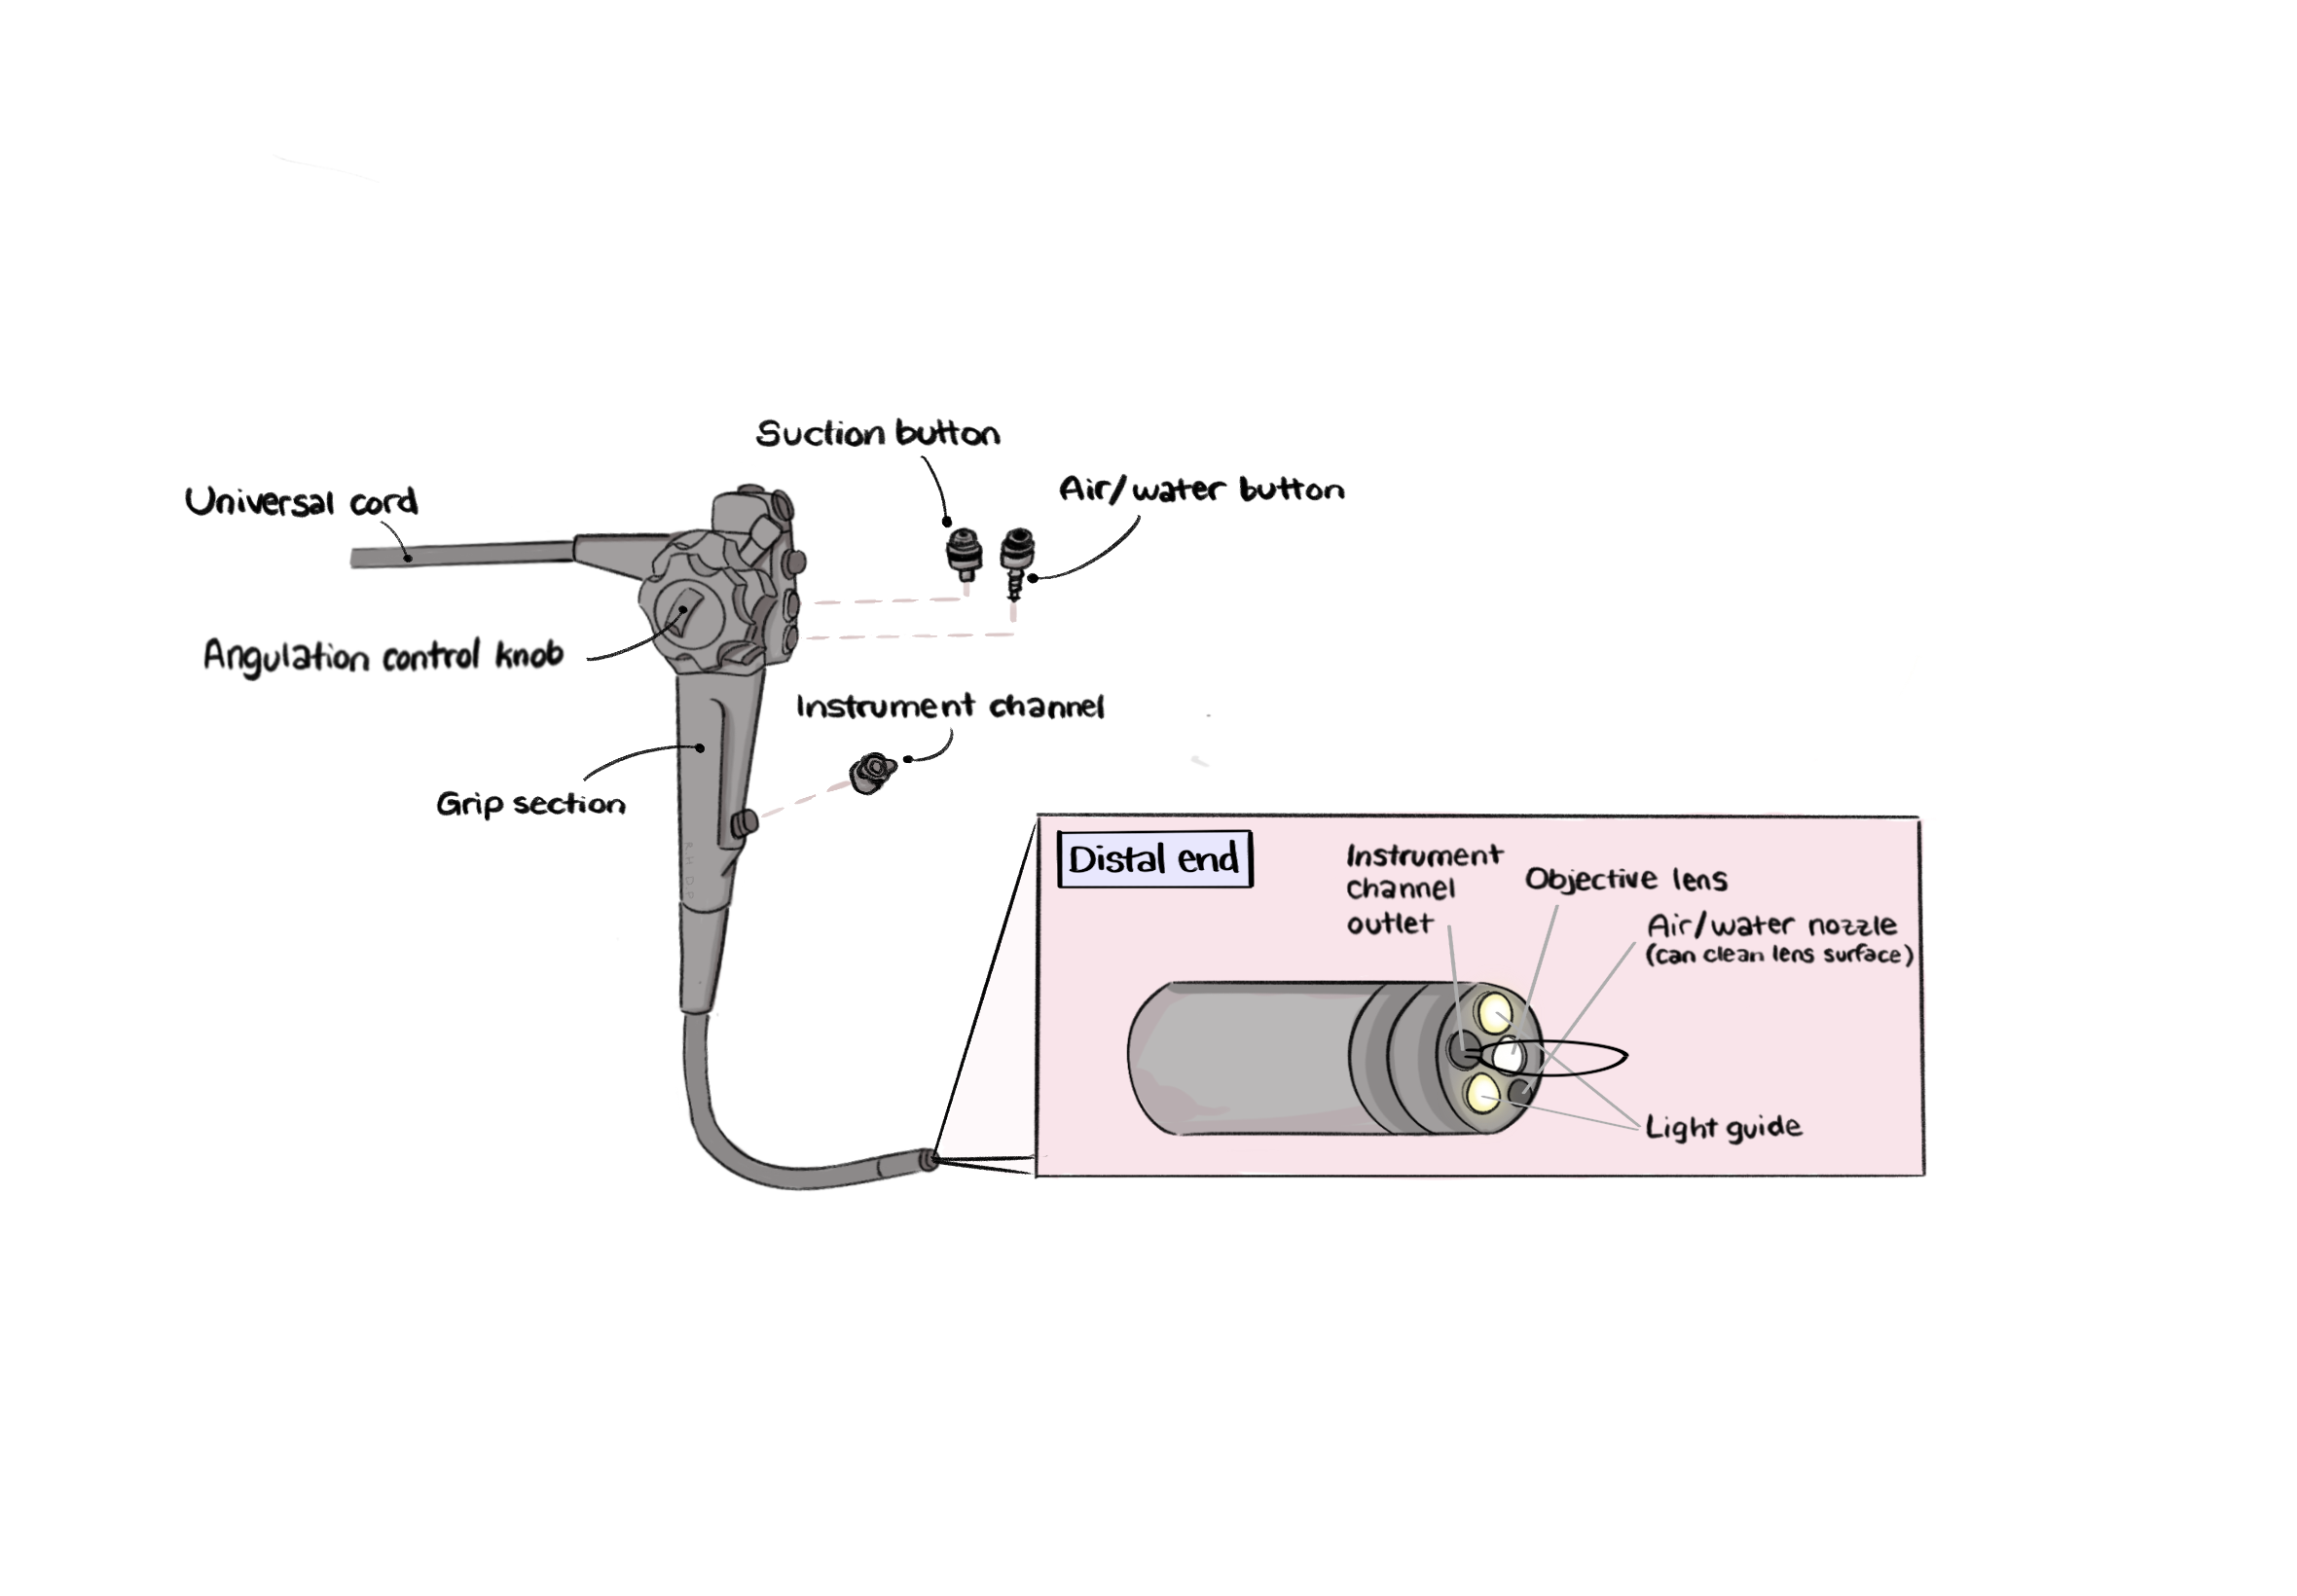
\includegraphics[width=1\linewidth,trim=2cm 6cm 6cm 5cm,clip]{assets/illustration-endoscope.png}%
}
\caption{Endoscope Components.}
\label{fig:endoscope_components}
\end{figure}

A modern endoscope provides a \textbf{live video feed} in high definition. The operator can bend the tip using \textbf{tip deflection} controls to get the best viewing angle. Other useful features include \textbf{insufflation}, which blows air or CO\textsubscript{2} to open up the colon walls, and \textbf{suction} to clear any fluid that blocks the view. The \textbf{instrument channel} allows the doctor to insert different tools depending on what needs to be done. Good \textbf{image quality} and a steady hand make it much easier to spot small polyps and treat them safely.

\begin{figure}[H]
\centering
\setlength{\fboxsep}{4pt}
\fbox{%
	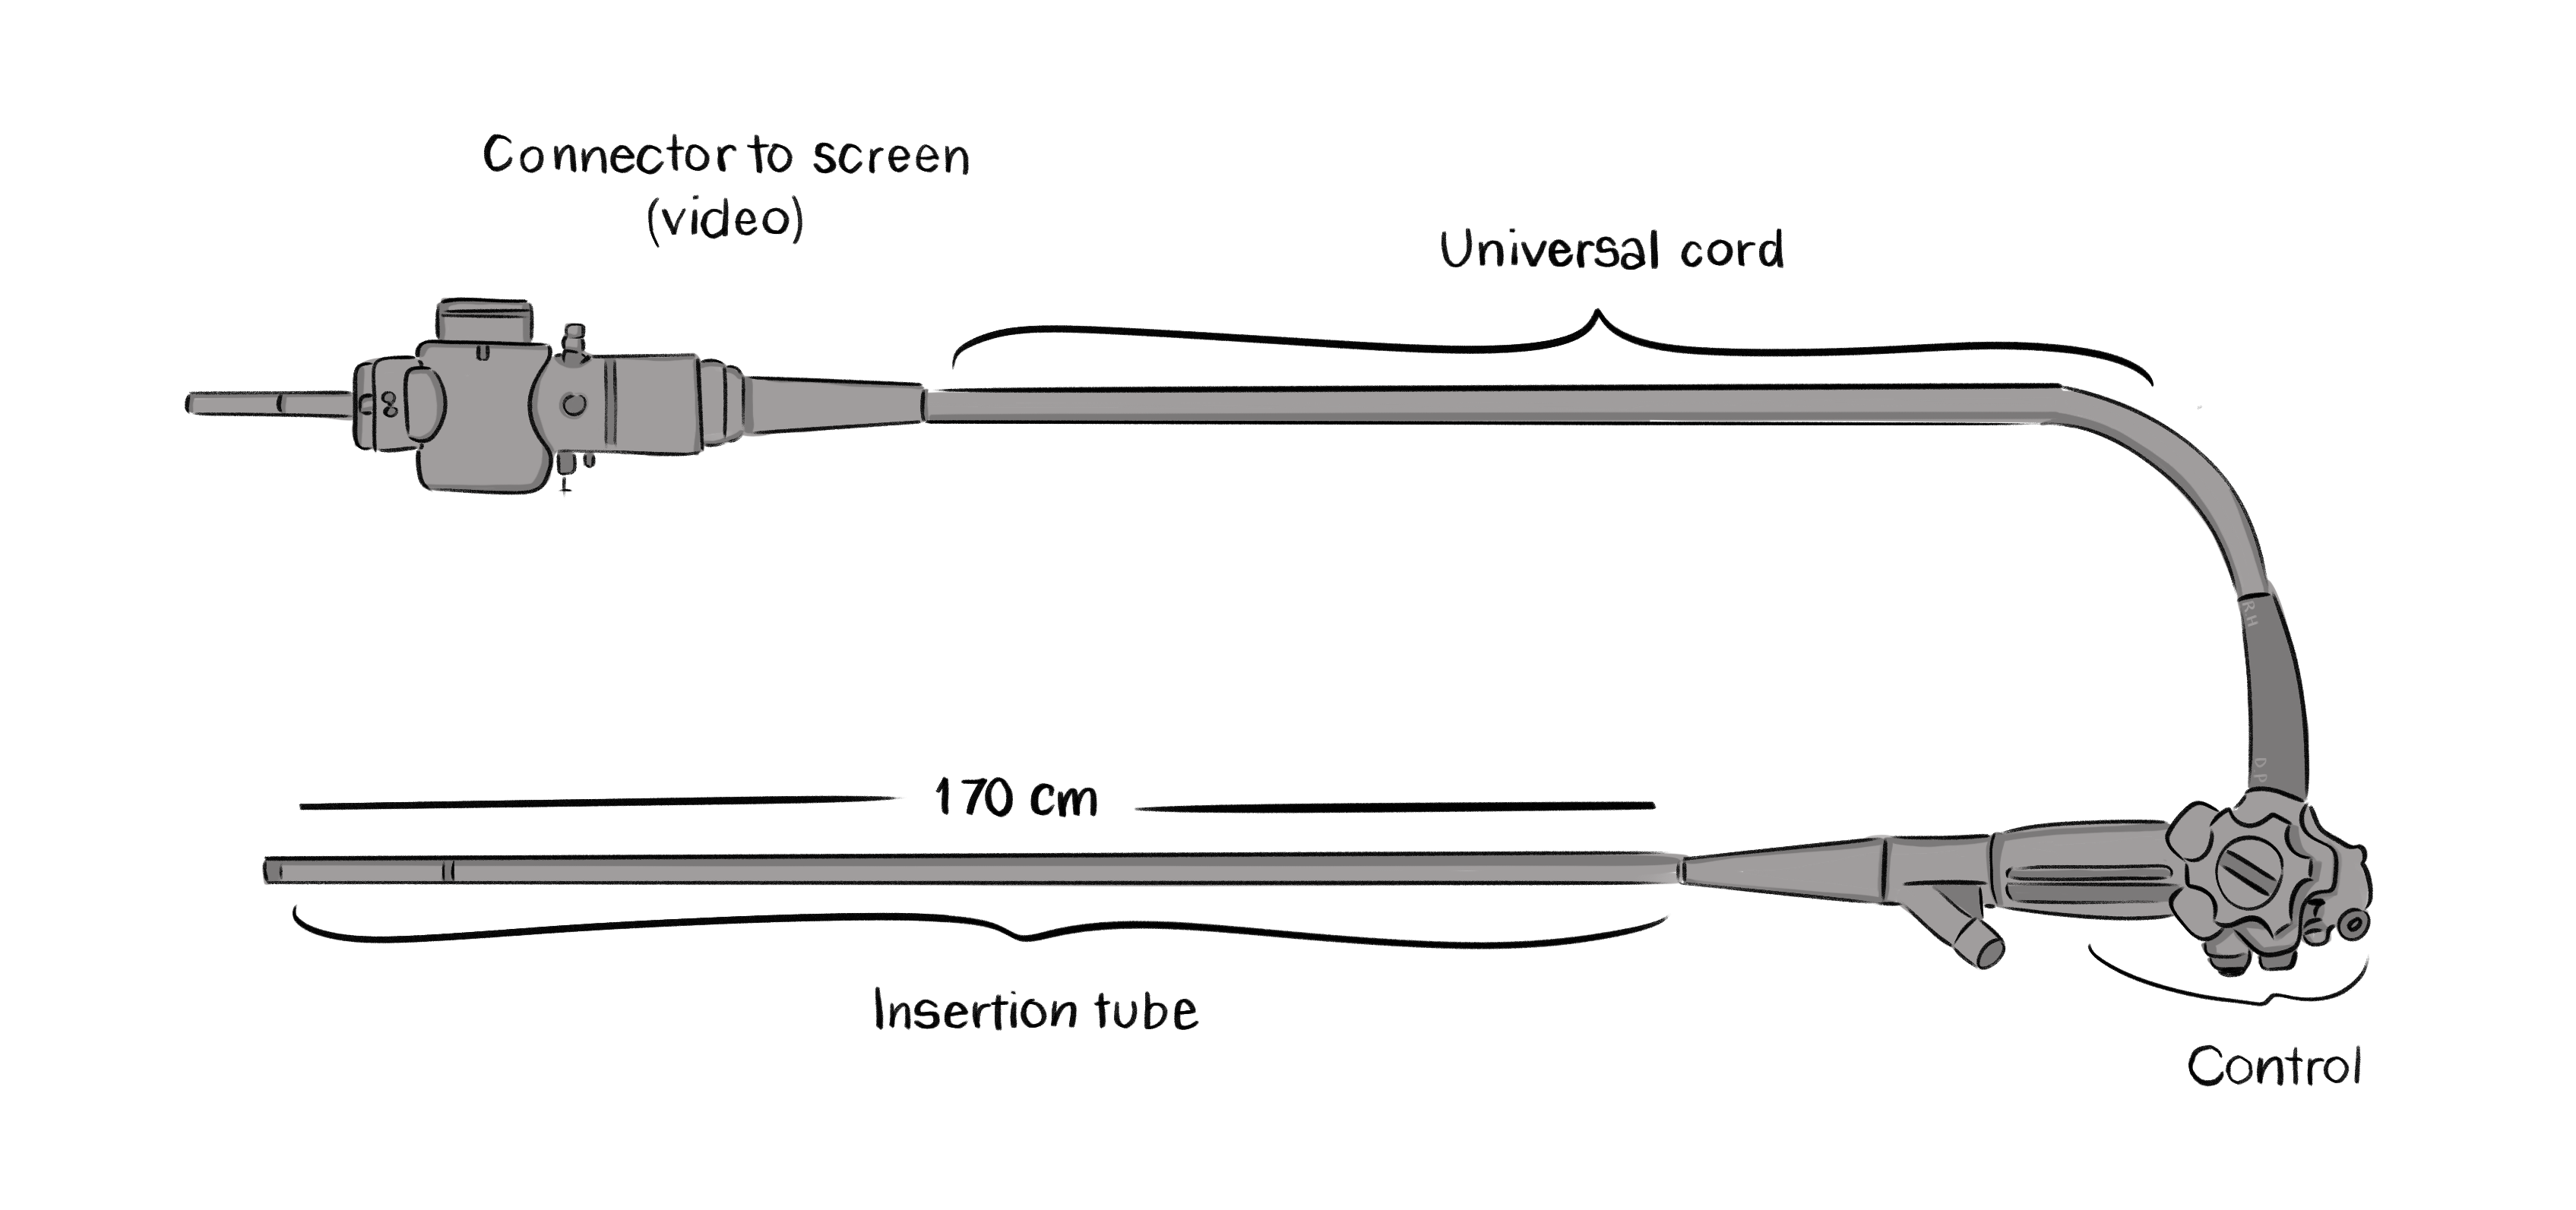
\includegraphics[width=1\linewidth]{assets/illustration-endoscope-dimensions.png}%
}
\caption{Endoscope Dimensions.}
\label{fig:endoscope_dimensions}
\end{figure}

The physical design of the endoscope is a careful balance between reach, flexibility, and patient comfort. The \textbf{insertion tube} is usually \textbf{130 to 170\,cm} long, which is enough to reach the full length of the colon. However, a longer tube can sometimes form loops inside the body, making it harder to control \cite{ferlitsch2017esge}. The \textbf{outer diameter} is typically \textbf{9 to 13\,mm}, and thinner scopes are more comfortable for the patient but may limit the size of instruments that can be used. The \textbf{working channel} (about \textbf{2.8 to 3.8\,mm} wide) decides which tools can fit through, such as snares, biopsy forceps, or retrieval nets. The \textbf{bending section} at the tip can move in multiple directions, which is essential for getting a clear, stable view of the colon wall.

Other features worth mentioning are the \textbf{control section}, where the operator adjusts the tip angle and manages instruments, and the built-in channels for \textbf{insufflation} and \textbf{suction}. For AI-assisted systems, things like \textbf{image quality}, low \textbf{latency}, and a stable video feed are very important because the computer needs a clear and consistent picture to work well.

\clearpage
\subsection{What is Colonoscopy?}

A \textbf{colonoscopy} is a medical procedure where the doctor uses an endoscope to look inside the entire colon and rectum. It is one of the most common procedures in gastroenterology, with over \textbf{19 million} colonoscopies performed every year in the United States alone \cite{lieberman2014screening}. It is used for three main purposes: \textbf{screening} for cancer, \textbf{diagnosing} problems like bleeding or inflammation, and \textbf{treating} issues such as removing polyps. Before the procedure, the patient needs good \textbf{bowel preparation} so that the doctor can see the lining of the colon clearly.

The main steps are simple to understand: first the patient is \textbf{prepared} and given \textbf{light sedation}, then the scope is \textbf{inserted and pushed forward} until it reaches the \textbf{cecum} (the start of the colon). After that, the doctor slowly \textbf{pulls the scope back} while carefully checking the walls for any lesions. If something is found, it can be \textbf{sampled or removed} right away. The whole process usually takes about \textbf{20 to 40 minutes}. Two important quality measures are the \textbf{cecal intubation rate} (how often the doctor reaches the cecum) and the \textbf{adenoma detection rate} (how often adenomas are found) \cite{corley2014adr}.

\begin{figure}[H]
\centering
\setlength{\fboxsep}{4pt}
\fbox{%
	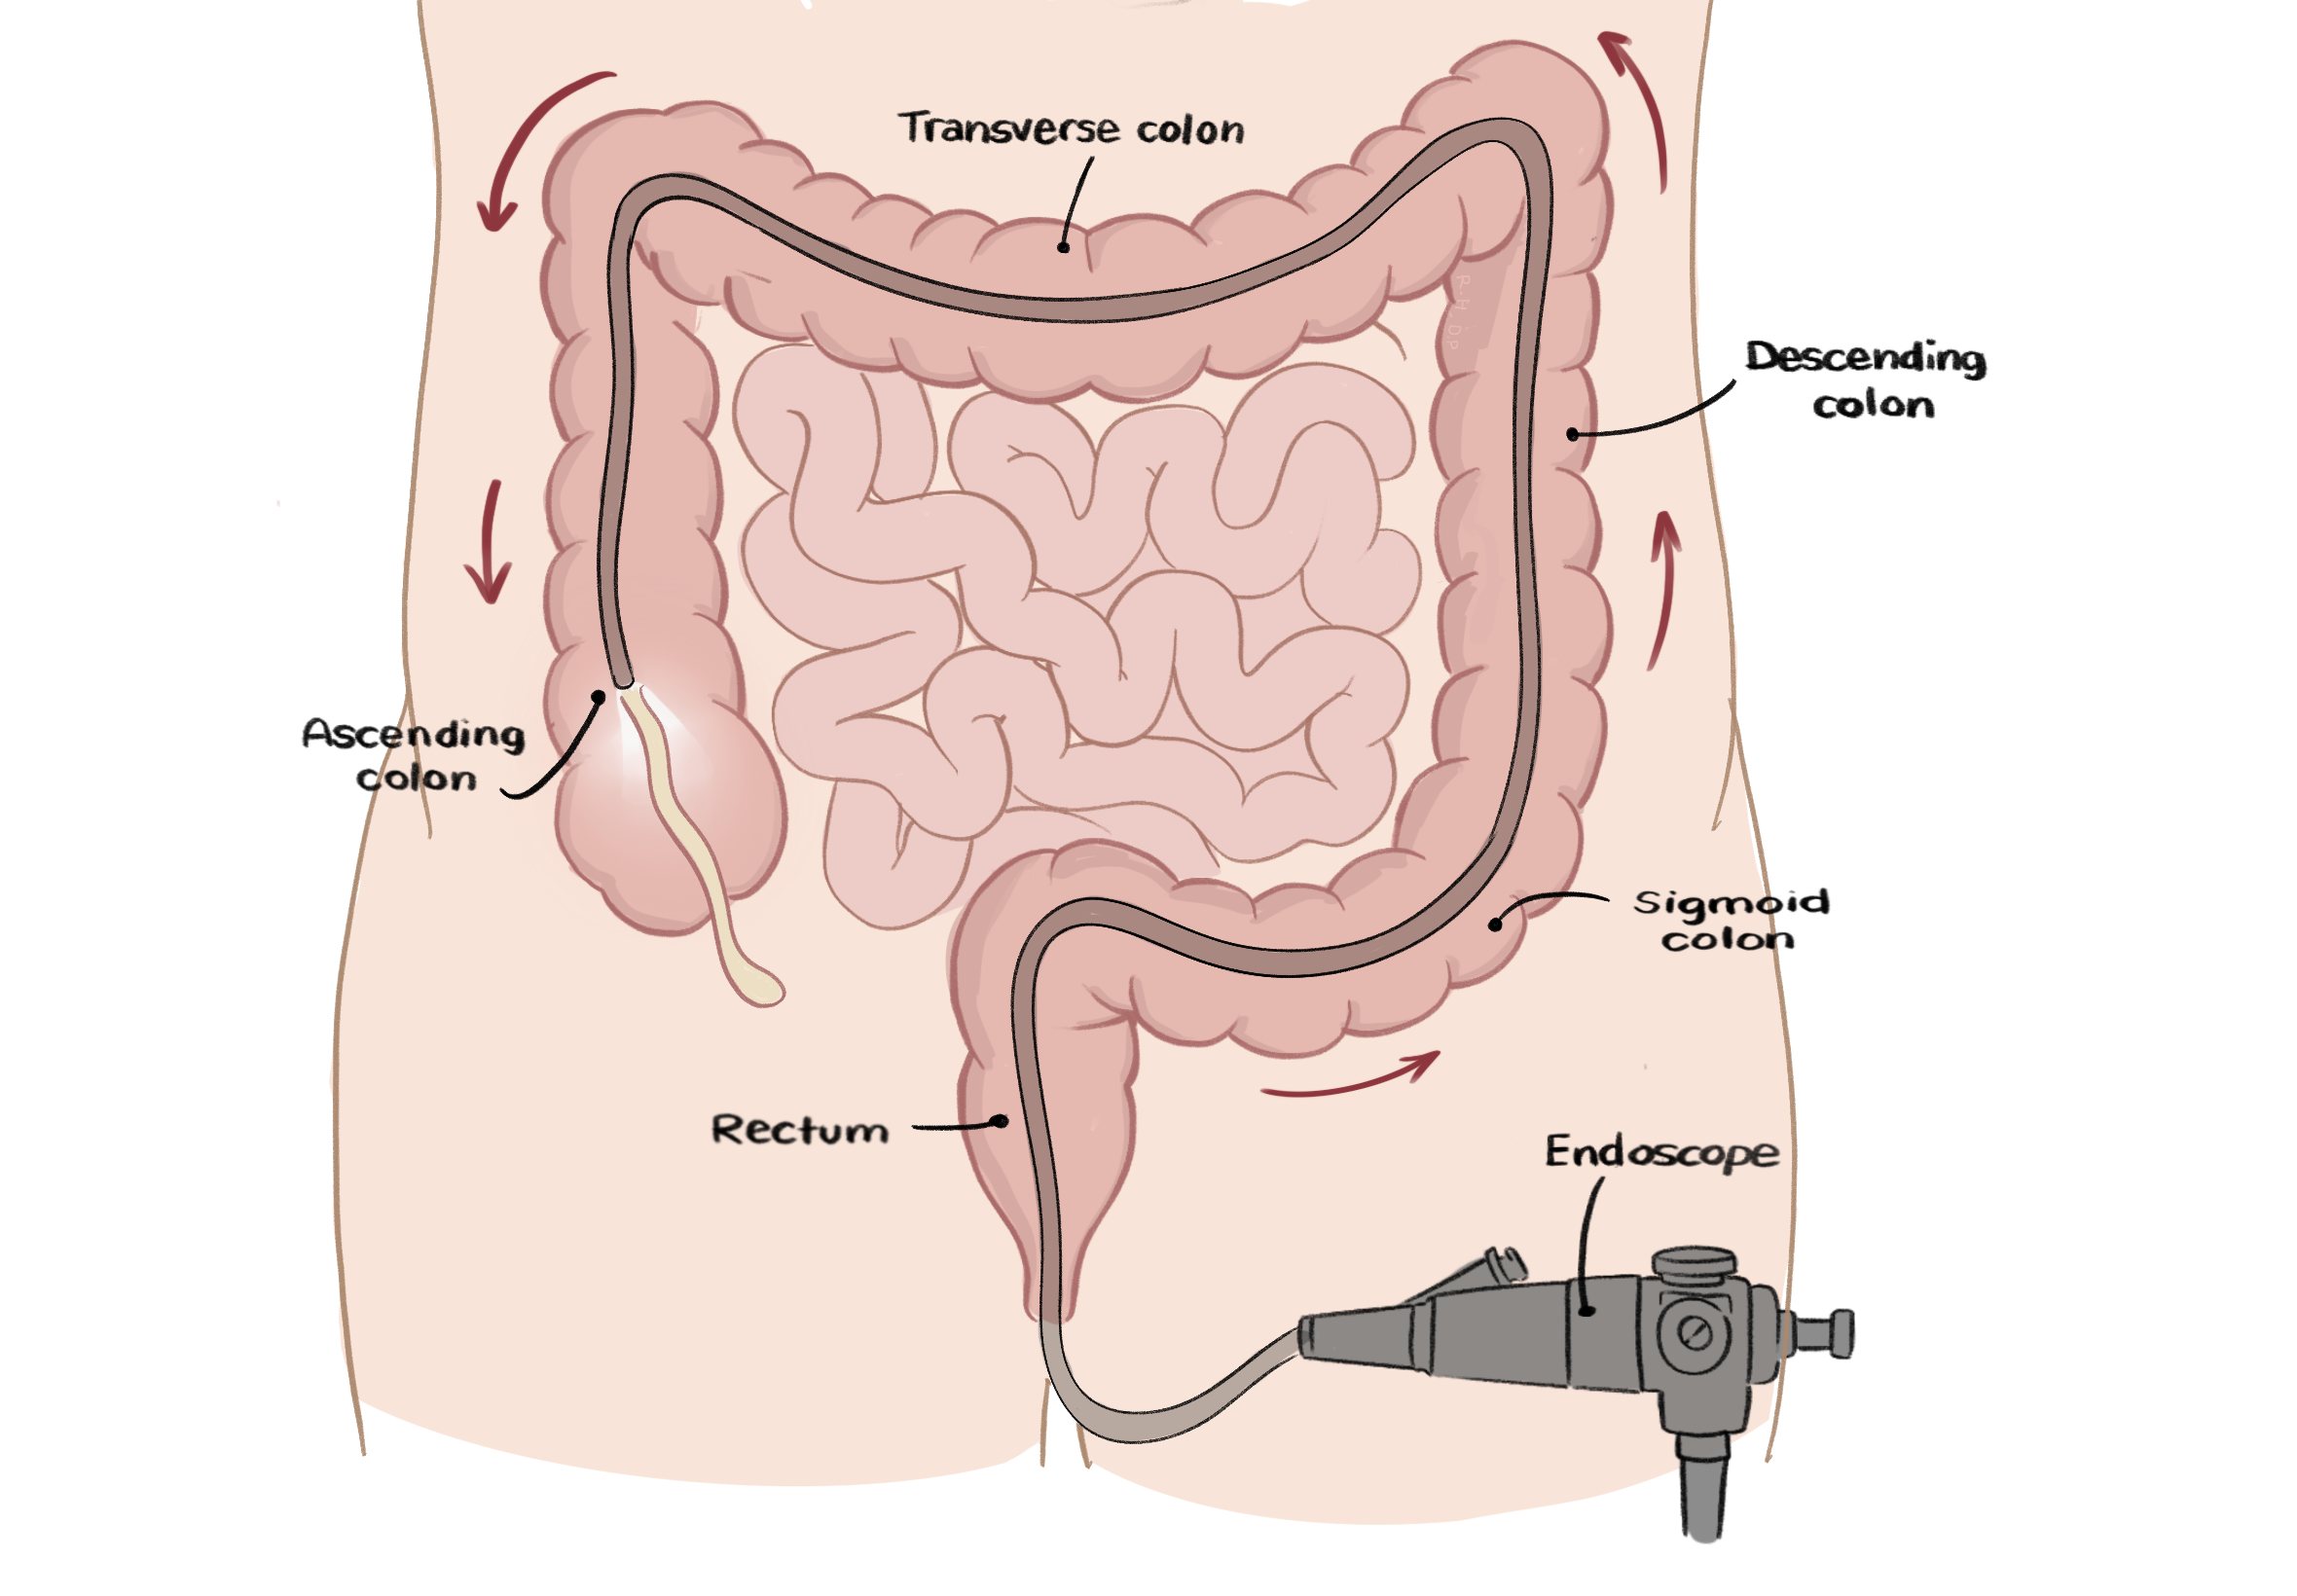
\includegraphics[width=1\linewidth,trim=1cm 0cm 2cm 0cm,clip]{assets/illustration-colonoscopy.png}%
}
\caption{Colonoscopy: scope view and instruments.}
\label{fig:colonoscopy_illustration}
\end{figure}

If a polyp is removed during the procedure, the doctor may use \textbf{clips} or \textbf{cautery} to stop any bleeding at the site. After the colonoscopy, the patient gets clear written instructions about what to watch for and when to come back. Follow-up depends on the \textbf{histology results} and the \textbf{size of the lesion} that was removed.

To put it simply: \textbf{endoscopy} is any procedure that uses a flexible camera to look inside the body. A \textbf{colonoscopy} is a specific type of endoscopy that examines the \textbf{colon} and \textbf{rectum}, and it is often done to screen for colorectal cancer or investigate symptoms. A \textbf{polypectomy} is when a \textbf{polyp} is actually removed during the colonoscopy.

\begin{figure}[H]
\centering
\setlength{\fboxsep}{4pt}
\fbox{%
	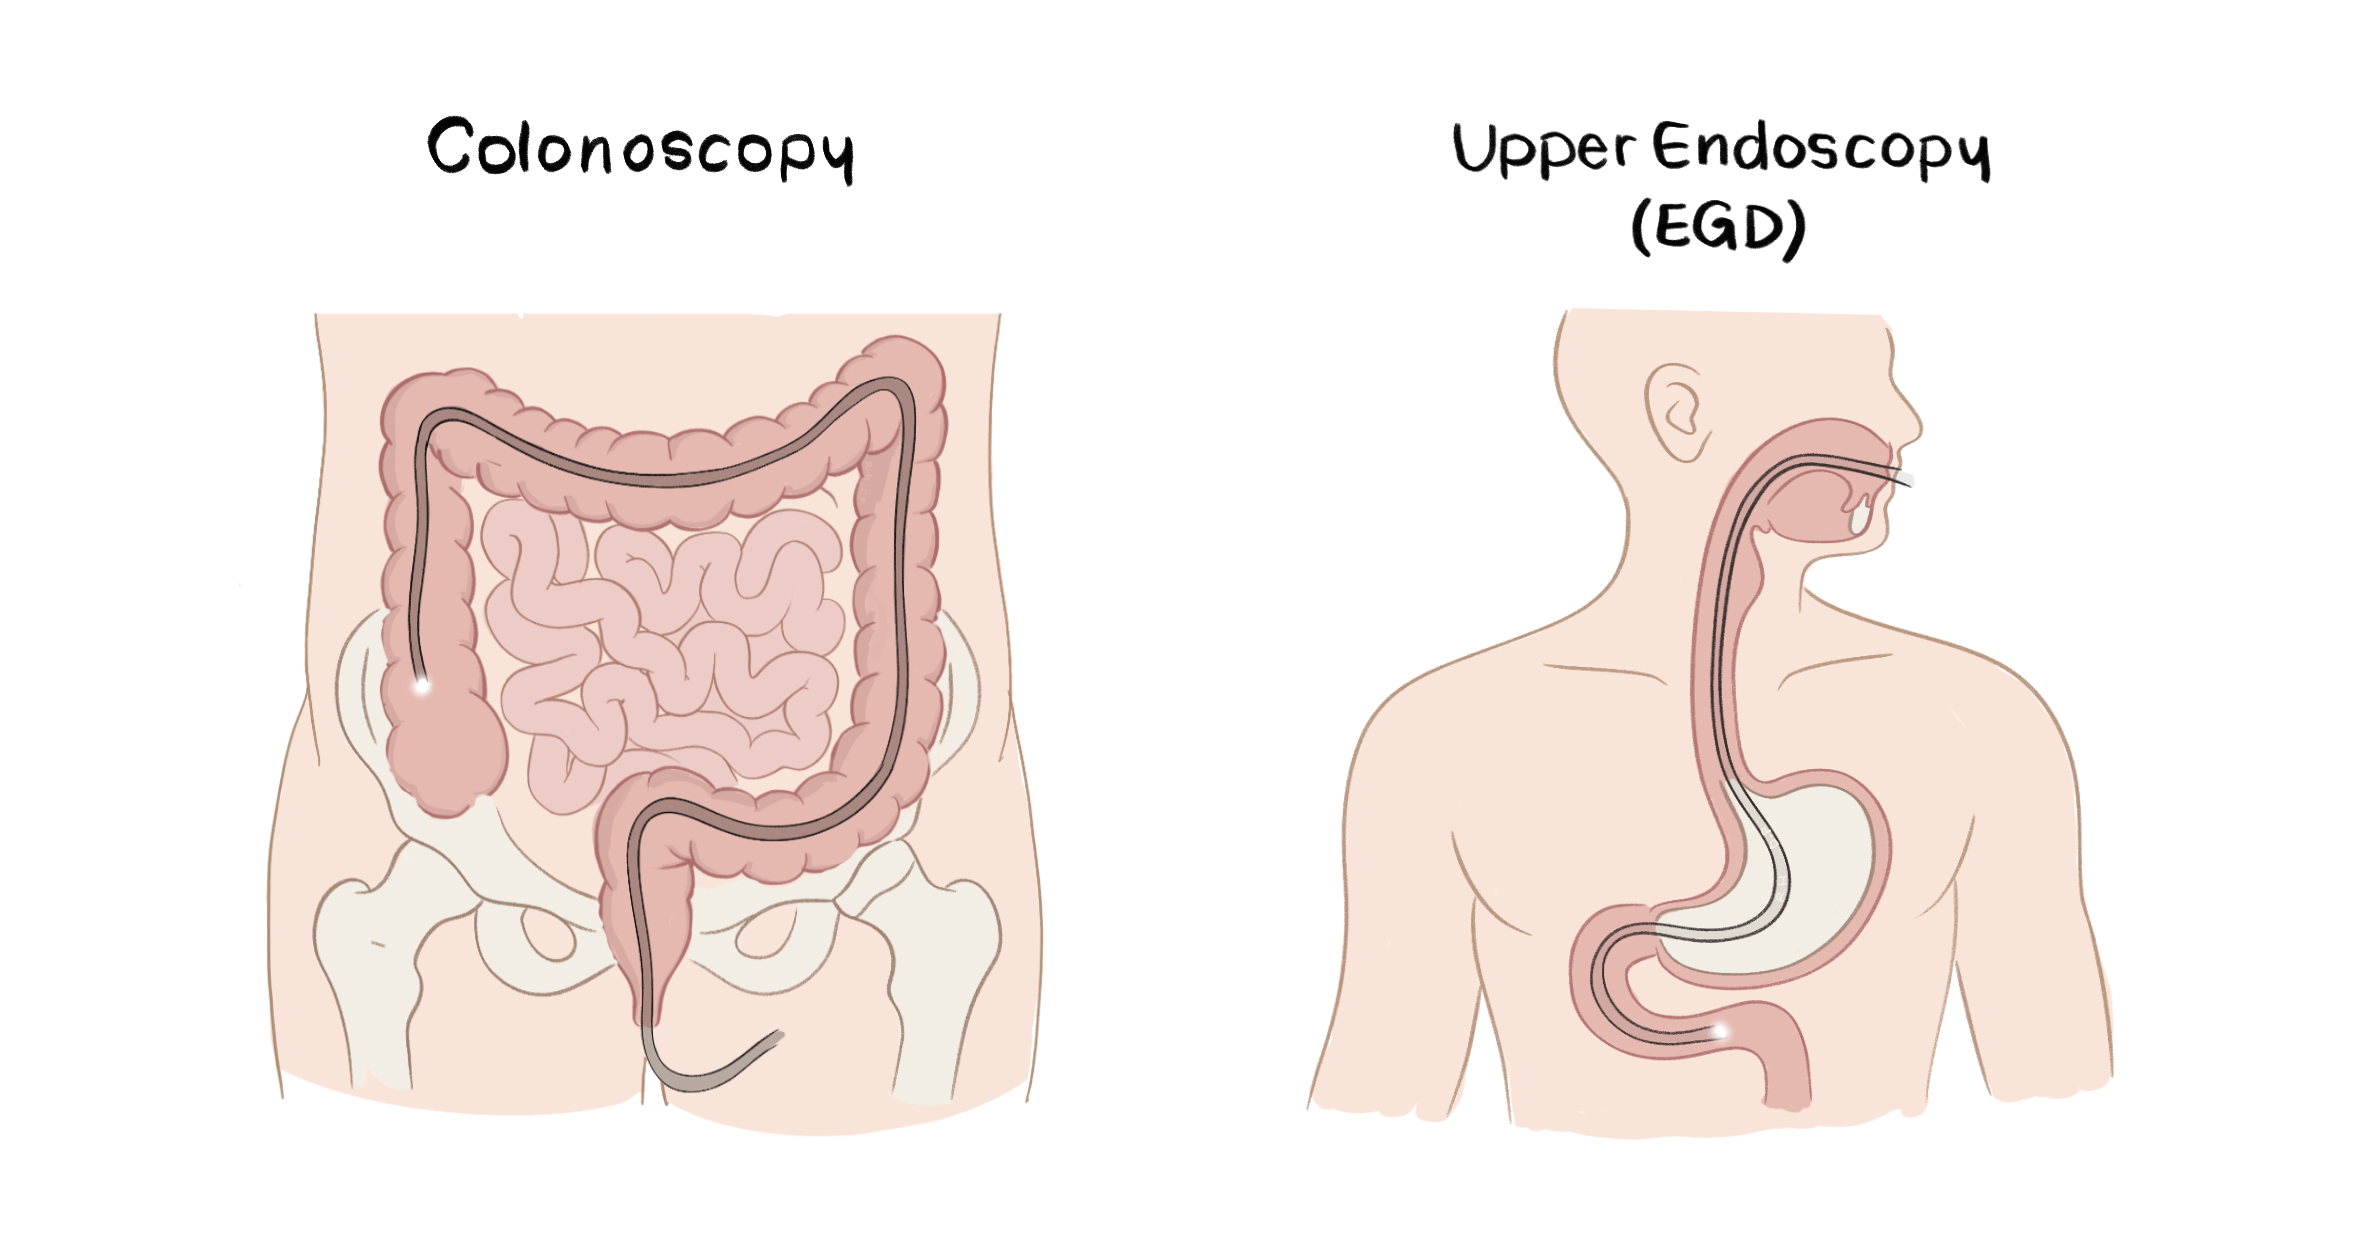
\includegraphics[width=1\linewidth]{assets/illustration-colonoscopy-vs-EGD.png}%
}
\caption{Colonoscopy vs Upper Endoscopy (EGD)}
\label{fig:colonoscopy_vs_upper-endoscopy}
\end{figure}

The abbreviation \textbf{EGD} stands for \textbf{EsophagoGastroDuodenoscopy}. Breaking it down: \textbf{Esophago} refers to the esophagus (the tube from the mouth to the stomach), \textbf{Gastro} refers to the stomach, \textbf{Duodeno} refers to the duodenum (the first part of the small intestine), and \textbf{-scopy} means looking or examining with a camera.


\clearpage
\subsection{What is Polypectomy?}
A \textbf{polypectomy} is the endoscopic \textbf{resection} (removal) of \textbf{colorectal polyps} during colonoscopy. Polyps may be benign, precancerous (\textbf{adenomas}), or malignant. Because appearance alone cannot exclude malignancy, \textbf{resection} and \textbf{histopathological assessment} are often recommended.

A \textbf{polypectomy} is therefore a subset of \textbf{endoscopy} - procedures that use an \textbf{endoscope} to visualise and sometimes treat the gastrointestinal tract.

Beyond screening, polypectomy is a \textbf{real-time} procedure that requires the operator to: \textbf{spot the lesion}, \textbf{judge its shape}, select the \textbf{resection method}, \textbf{position tools}, \textbf{manage bleeding risk}, and ensure the \textbf{removal is complete}. This is why reliable \textbf{perception} and safe \textbf{decision-making} are essential.

\begin{figure}[H]
\centering
\fbox{
	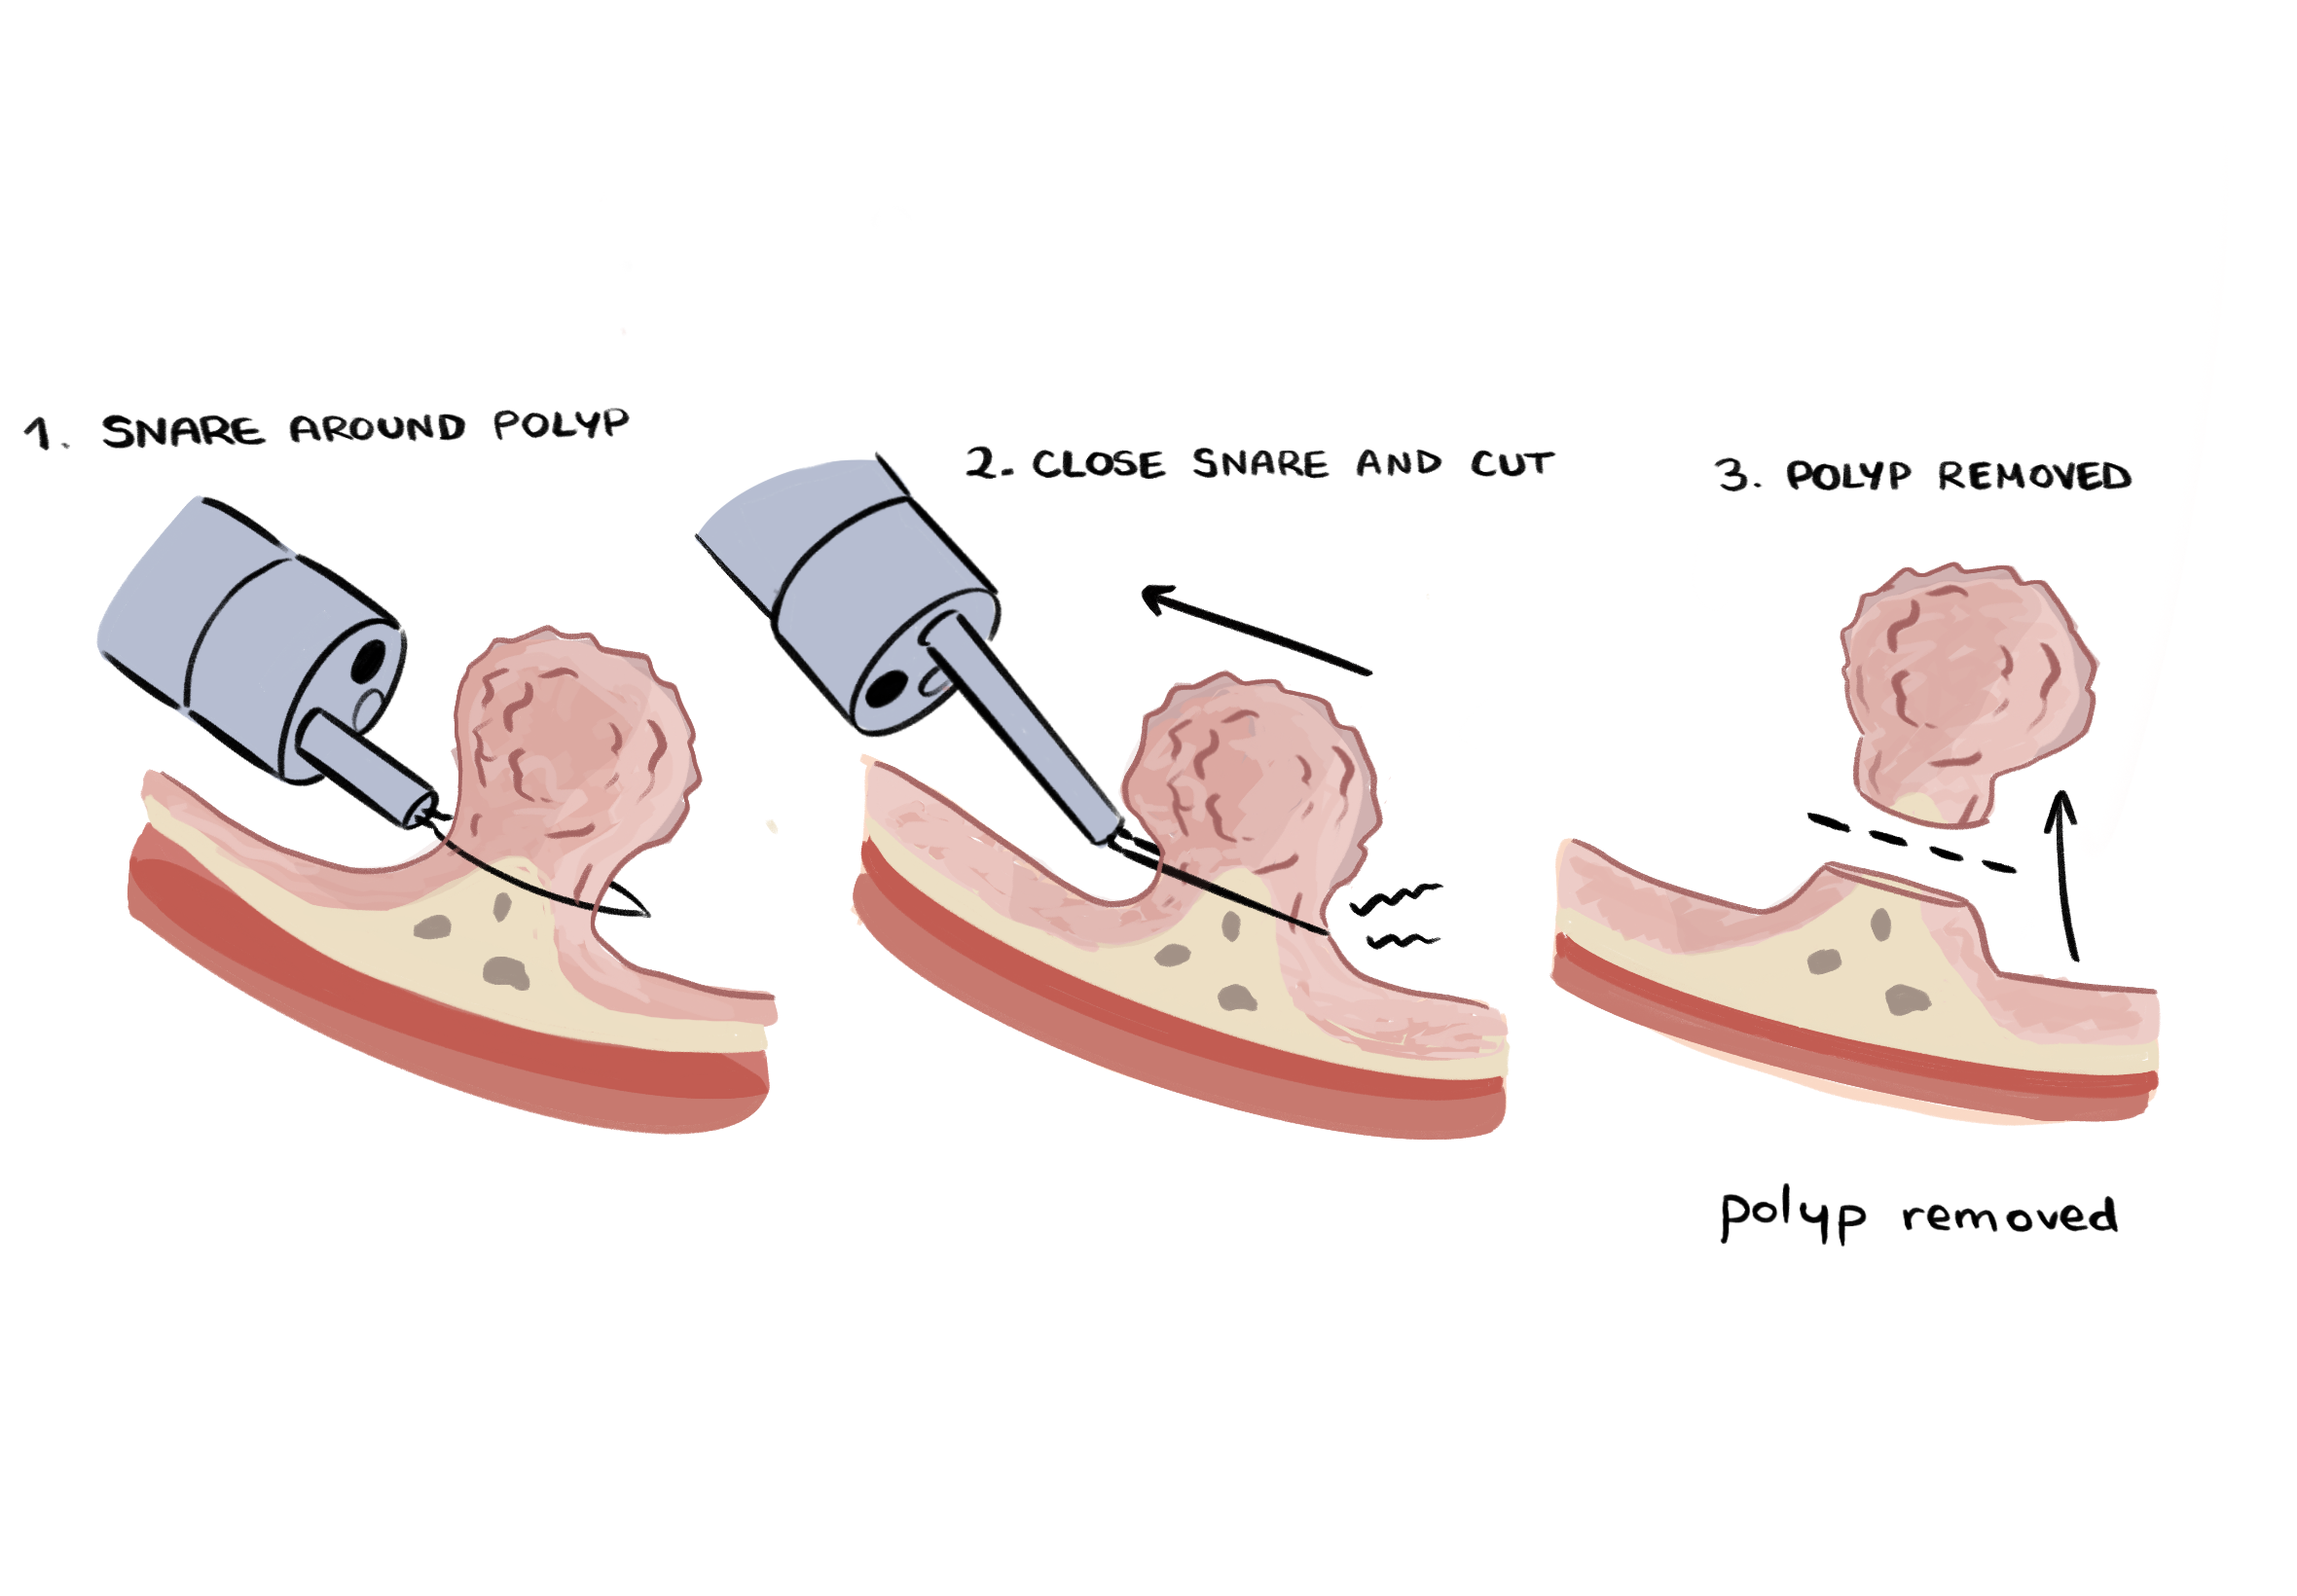
\includegraphics[width=1\linewidth,trim=0 8cm 0 3cm,clip]{assets/illustration-polyp-extraction.png}%
}
\caption{Polypectomy extraction illustration (scope tip, snare, lesion).}
\label{fig:polypectomy_extraction}
\end{figure}

After the polypectomy the operator will \textbf{inspect the site} for bleeding and check the \textbf{resection margins}. Minor bleeding is treated with \textbf{clips} or \textbf{coagulation} as needed. The patient receives brief \textbf{after-care advice} and clear instructions about signs that need urgent review.


\clearpage
Resection choice depends on lesion shape (\textbf{pedunculated} vs \textbf{sessile/flat}), size, visibility, access angle, tissue scarring, and bleeding risk \cite{ferlitsch2017esge,ESGE2024_Polypectomy_Update}.

Common options:
\begin{itemize}
\item \textbf{Cold snare}: no electrocautery; safe for small polyps and lowers thermal injury risk.
\item \textbf{Hot snare}: uses electrocautery for cutting and haemostasis; useful for some larger or bleeding lesions but adds thermal risk.
\item \textbf{Submucosal injection + snare (EMR)}: inject fluid under the lesion to lift it, then snare; good for larger sessile lesions and can be done piecemeal.
\item \textbf{ESD}: dissection in the submucosal layer for en‑bloc removal of complex lesions; offers better margins but is slower and technically demanding.
\end{itemize}


\begin{figure}[H]
\centering
\fbox{
	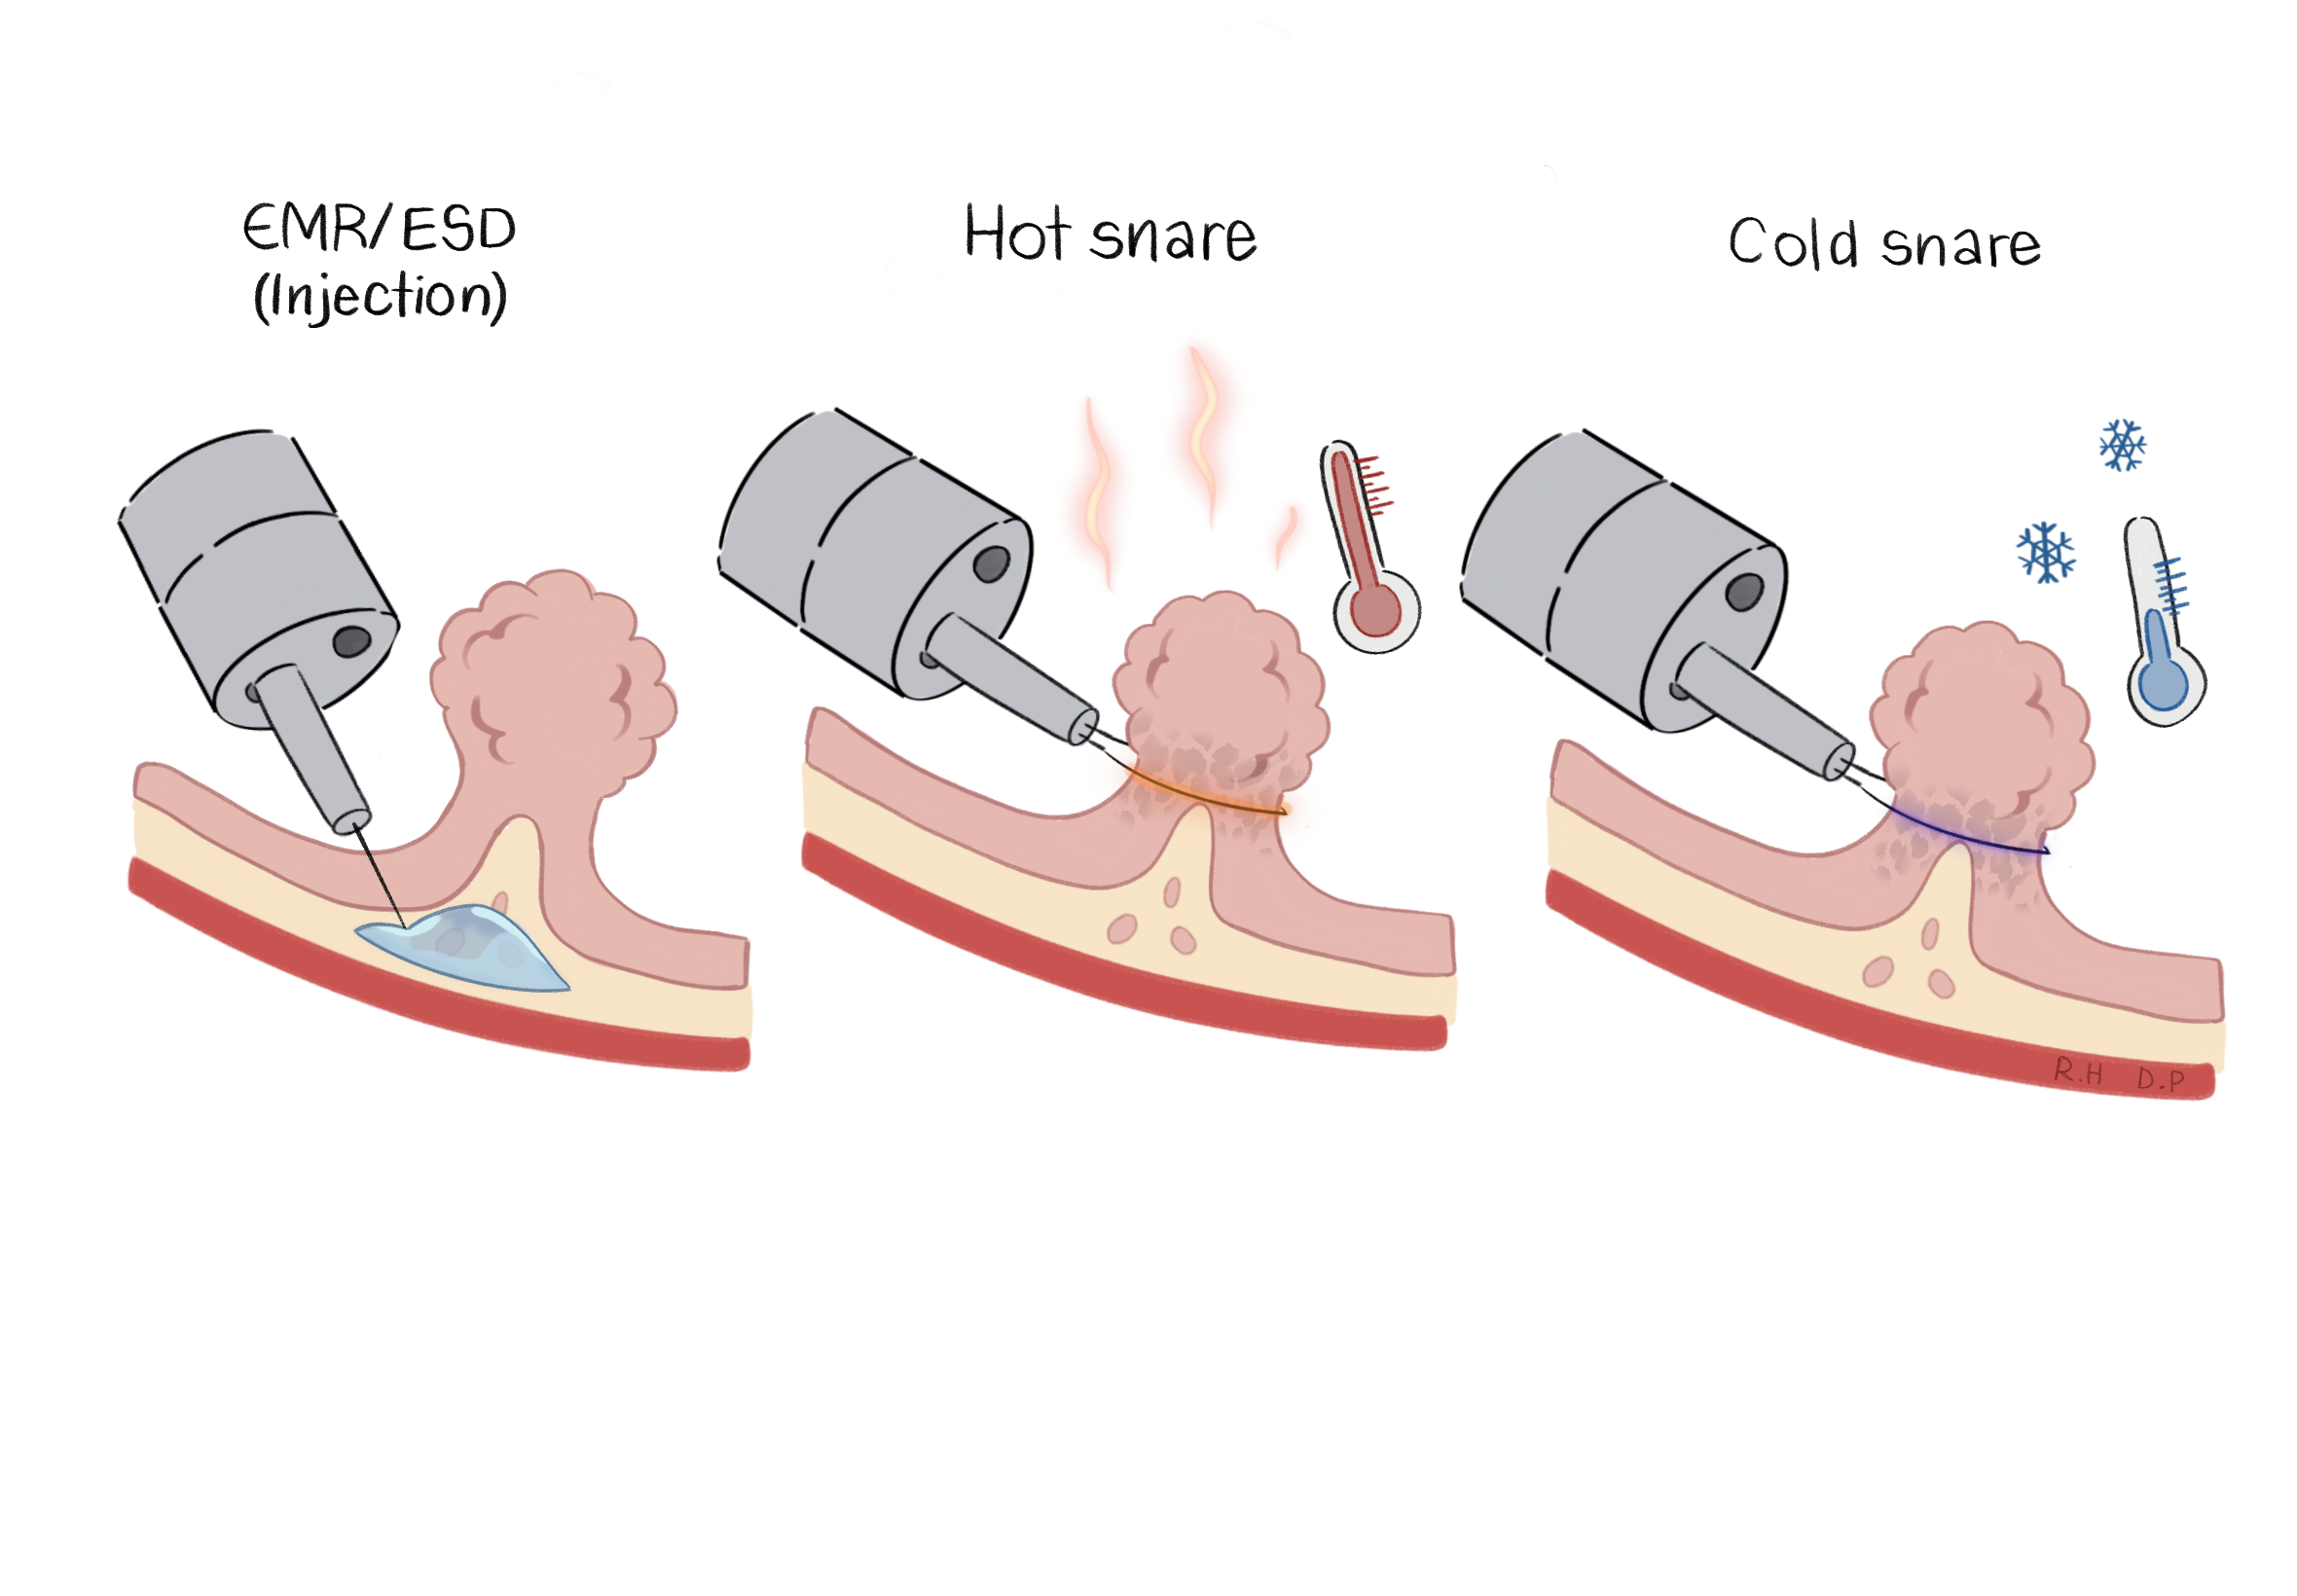
\includegraphics[width=1\linewidth,trim=0 8cm 0 3cm,clip]{assets/illustration-cutting-technique.png}%
}
\caption{Polypectomy cutting techniques (hot, cold, injection).}
\label{fig:polypectomy_cutting_techniques}
\end{figure}

When to prefer injection: if the lesion is flat or there is concern about deep invasion or scarring, a \textbf{submucosal injection} improves safety and helps achieve a clean resection plane. Cold snare is preferred for small, non‑fibrotic polyps because it reduces delayed bleeding in many trials \cite{Chang2023_AnnInternMed,Liu2023_IntJColorectalDis}.

Choosing a method balances \textbf{completeness} (low recurrence) and \textbf{procedural risk} (bleeding, perforation) and depends on operator skill. See ESGE guidance and ESD reviews for indications and technique \cite{ferlitsch2017esge,PimentelNunes2015_ESGE_ESD,ESGE2024_Polypectomy_Update}.







\clearpage
\section{Basics of Artificial Intelligence}
\label{sec:basics_artificial_intelligence}

\subsection{What is AI and Why Does It Matter Now}

\textbf{Artificial Intelligence} (AI) is the idea of making computers do things that normally need human thinking, like recognising objects in a picture, understanding language, or making decisions in complex situations \cite{goodfellow2016deep}. It is not one single technology but a big family of methods that all share the same goal: teach machines to learn from data and improve over time.

\begin{figure}[H]
\centering
\setlength{\fboxsep}{4pt}
	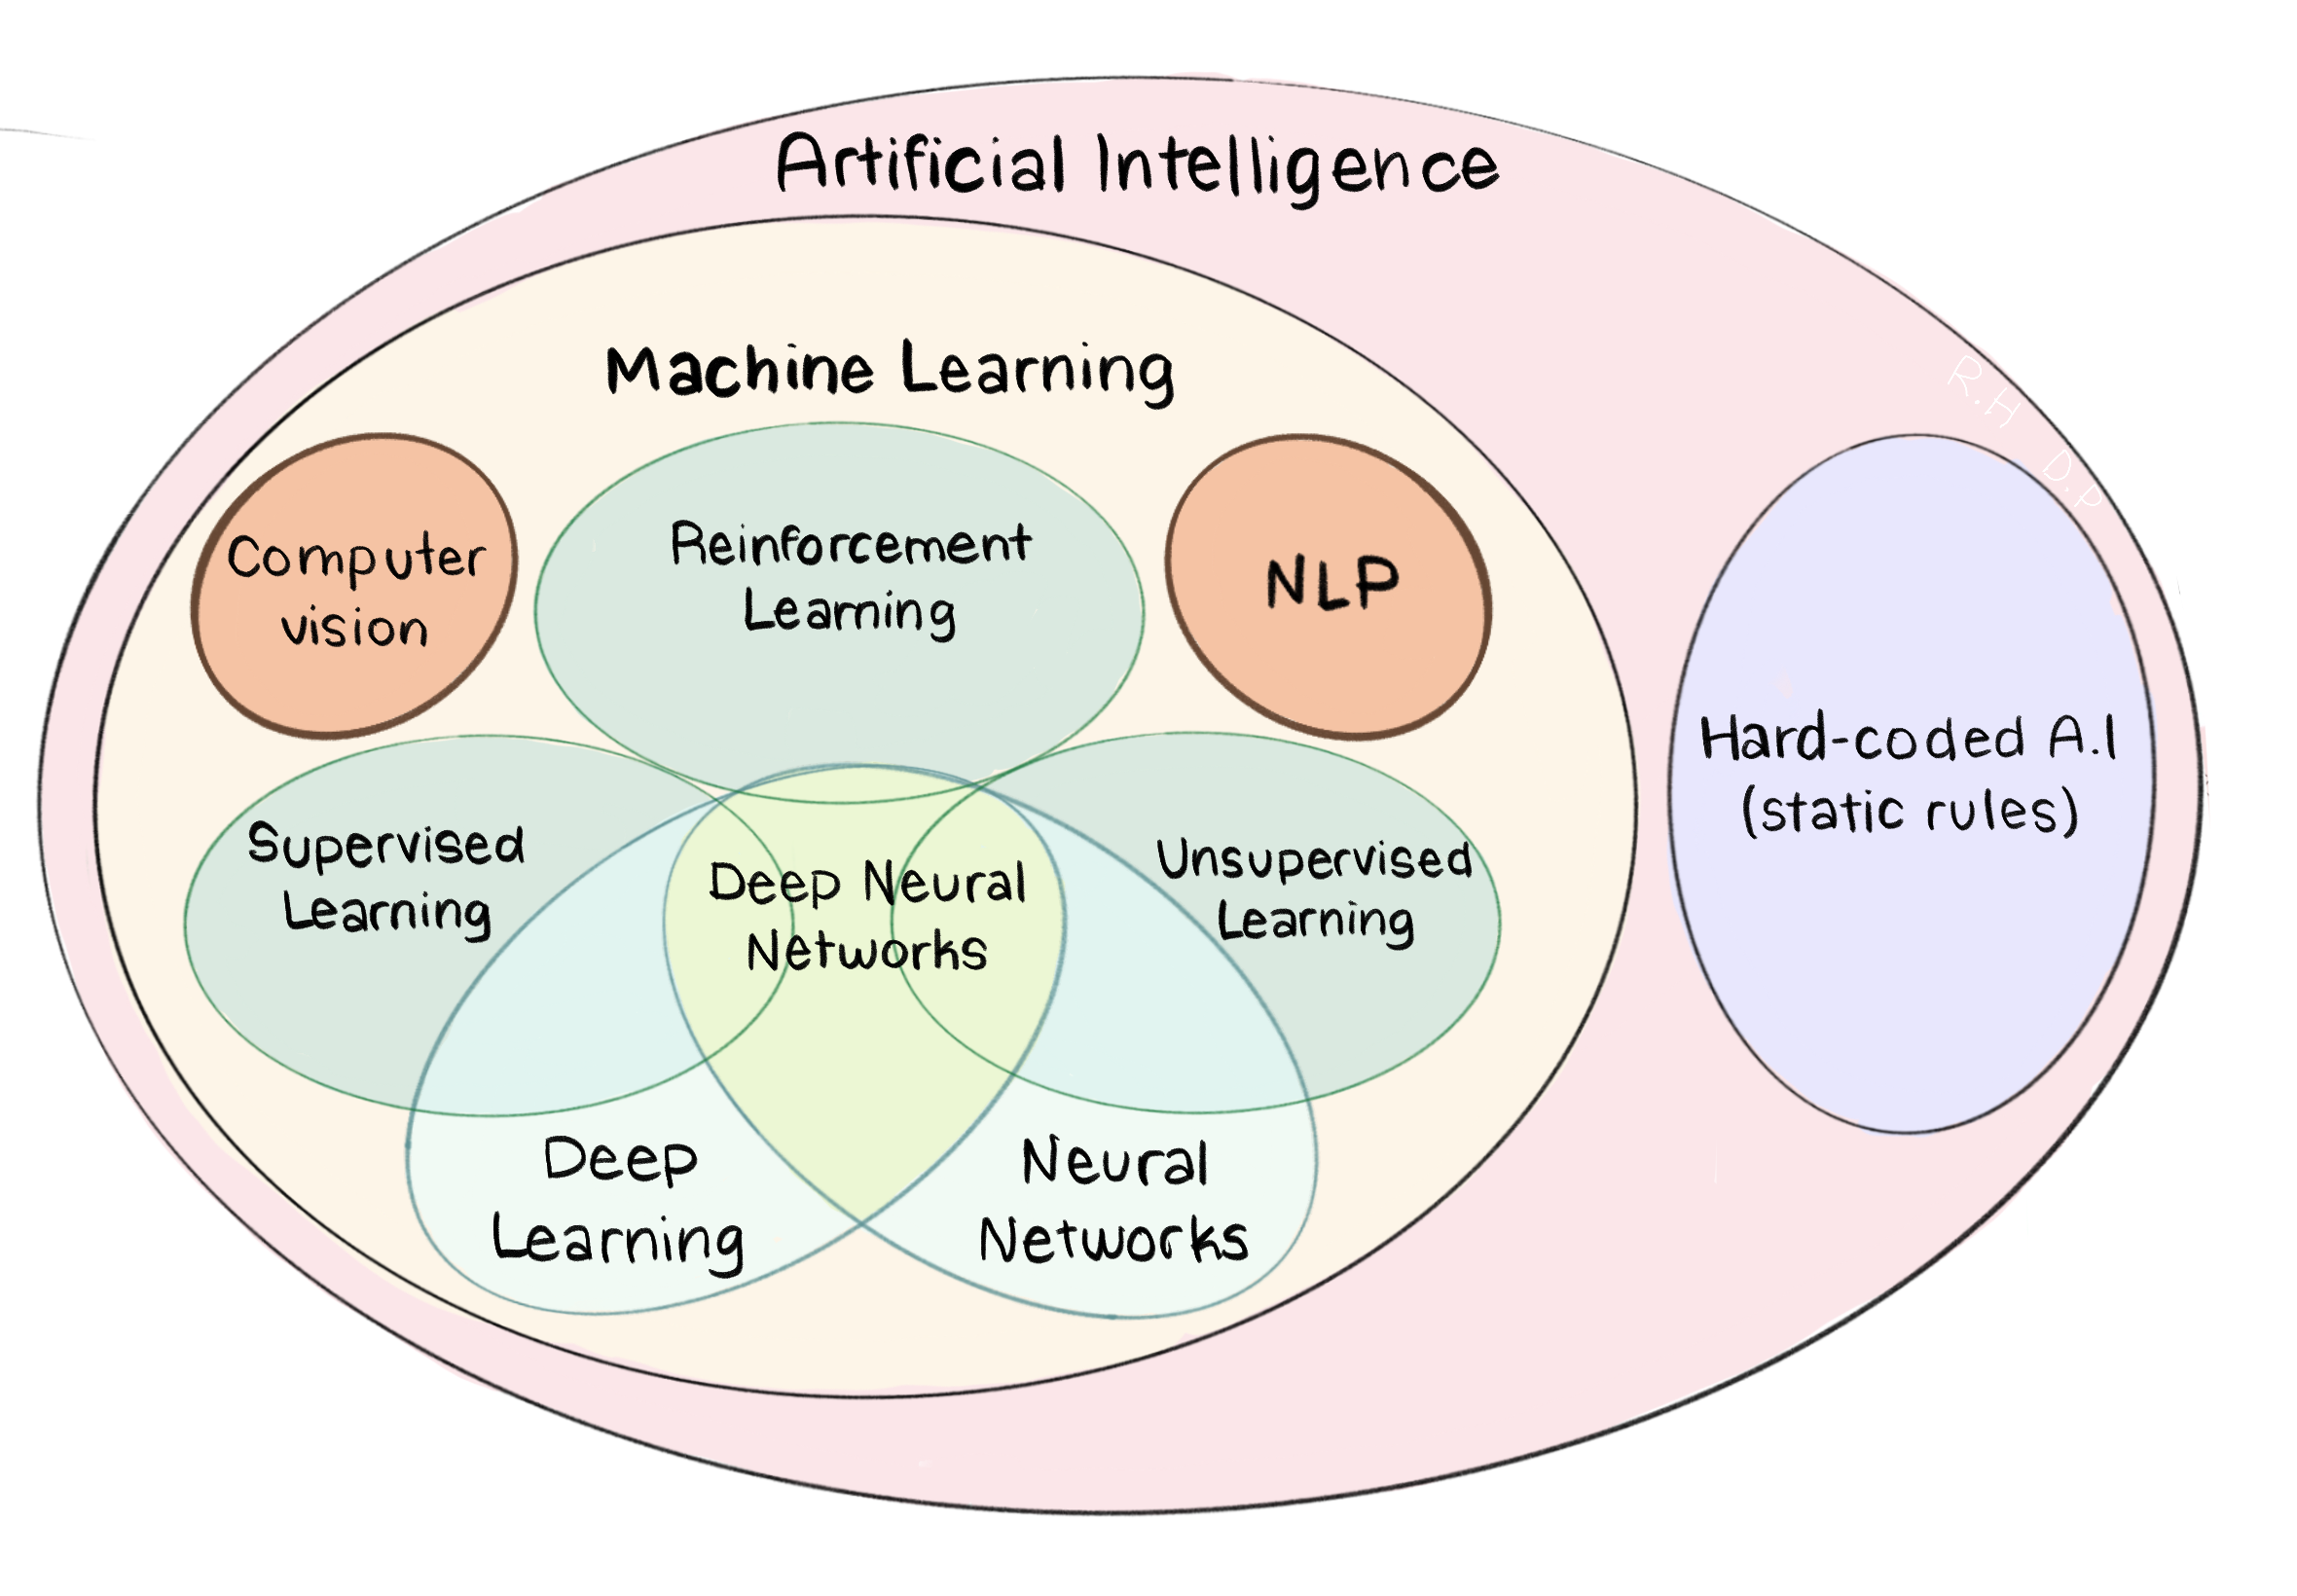
\includegraphics[width=1\linewidth]{assets/diagram-a.i-venn.png}%
\caption{How the main fields of AI relate to each other.}
\label{fig:ai_venn}
\end{figure}

The field has been around since the 1950s, but it really took off in the last decade thanks to three things happening at the same time: much bigger \textbf{datasets}, much faster \textbf{hardware} (especially GPUs), and better \textbf{algorithms} like deep neural networks \cite{litjens2017dlSurvey}. To give an idea of how fast things are moving, the famous \textbf{AlphaGo} system by DeepMind beat the world champion in the board game Go in 2016, a task that many researchers thought was still decades away \cite{silver2016alphago}. That moment really showed the world what modern AI could do.

Inside the AI family, there are a few important subfields that we use in this project:

\begin{itemize}
\item \textbf{Machine Learning (ML):} methods that let a computer learn patterns from data without being told exactly what to look for.
\item \textbf{Deep Learning (DL):} a part of ML that uses neural networks with many layers, and it is especially good at working with images and video.
\item \textbf{Computer Vision (CV):} techniques for understanding what is in an image or a video, like detecting objects or tracking motion.
\item \textbf{Deep Reinforcement Learning (Deep RL):} a way for an agent to learn by trying actions and getting feedback (rewards or penalties) from the environment.
\end{itemize}



What makes AI so exciting right now is that these subfields are starting to work together. In our project, for example, we use deep learning to understand what the camera sees (that is the computer vision part), and then deep reinforcement learning to decide what to do next. This combination is what makes intelligent agents possible.

\subsection{How AI is Already Used in Medicine and Endoscopy}

AI is not just a research topic anymore. It is already being used in real hospitals. In radiology, AI systems help doctors read X-rays and CT scans faster. In pathology, they help analyse tissue samples. And in \textbf{endoscopy}, which is the field that interests us most, AI is making a real difference.

One of the most exciting results in recent years came from clinical trials that tested \textbf{computer-aided detection} (CADe) systems during colonoscopy. These systems run in real time and highlight suspicious areas on the screen to help the doctor spot polyps. A large randomised trial by Wang et al. found that using a CADe system increased the \textbf{adenoma detection rate} from \textbf{20\,\%} to \textbf{29\,\%}, which is a big improvement \cite{wang2019cade}. Another trial by Repici et al. confirmed similar results, showing that AI-assisted colonoscopy finds more polyps without making the procedure longer \cite{repici2020cade}.

These systems are mostly focused on \textbf{detection}, meaning they help the doctor see the polyp. But the next big question is: can AI also help with the \textbf{treatment} itself? That is where our project comes in.

A good survey by Nazarian et al. looked at many studies on AI for polyp detection and characterisation, and found that deep learning models can reach a \textbf{sensitivity above 90\,\%} in detecting colorectal polyps from endoscopic images \cite{nazarian2021jmir}. That means the technology is already quite reliable for spotting lesions. But actually removing them safely is a very different challenge.

\subsection{What Our Agent Needs to Do: Navigate and Extract}

In this project, we are not building a polyp detector. Instead, we are building an agent that can \textbf{act} inside a simulated colon. The agent has two main jobs:

\begin{itemize}
\item \textbf{Navigate:} the agent must guide the endoscope tip through the colon, avoid hitting the walls, keep a clear view, and reach the area where the polyp is located. This is like driving through a narrow, winding tunnel where the walls are soft and the lighting keeps changing.
\item \textbf{Extract:} once the agent is close enough to the polyp, it needs to use a snare tool to grab and remove it. This means extending the snare, positioning it around the polyp, and closing it at the right moment without damaging the surrounding tissue.
\end{itemize}

Both tasks are \textbf{sequential}, which means each action affects what happens next. A bad move now can make the next step much harder. That is exactly the kind of problem where deep reinforcement learning works well, because the agent learns to think ahead and not just react to the current frame.

The agent uses a \textbf{CNN} to understand what the camera sees, an \textbf{LSTM} to remember what happened a few steps ago, and \textbf{PPO} (a deep reinforcement learning algorithm) to decide what to do next. We will explain each of these in the following sections, starting with deep reinforcement learning.

\clearpage
\section{Reinforcement Learning for Sequential Decision-Making}
\label{sec:reinforcement_learning}

\subsection*{Introduction}
Reinforcement Learning (\textbf{RL}) is a way for an agent to learn by trying actions and getting feedback. If the action helps, the agent gets a better reward. If not, it learns and tries again. That simple loop makes RL a good fit for tasks that happen step by step, like moving an endoscope, keeping the view stable, or controlling a snare \cite{sutton2018reinforcement}.

In this work, RL is not just theory in a textbook. It is the idea behind an agent that must act in a messy, changing scene and still stay safe. We use modern policy methods, especially \textbf{Proximal Policy Optimization (PPO)}, because they are stable and work well with neural networks \cite{schulman2017ppo}. Classic deep RL results such as \textbf{DQN} and \textbf{AlphaGo} show how far the field has come \cite{mnih2015dqn,silver2016alphago}.

\begin{figure}[h]
\centering
\fbox{\parbox[b][3.8cm][c]{0.9\linewidth}{\centering Placeholder: RL overview showing agent, environment, state, action, and reward}}
\caption{Main RL components and feedback loop (placeholder).}
\label{fig:rl_components}
\end{figure}

\subsection{The RL Loop}
The RL loop is easy to remember: the agent sees a \textbf{state}, chooses an \textbf{action}, and gets a \textbf{reward}. Then the environment changes, and the next state appears. This repeats many times. The goal is not to win one step, but to collect the best total reward over time.

For our project, this loop matters because the best action now may depend on what happened a few frames ago. A small move can make the next image clearer, or a wrong move can hide the lesion. RL helps the agent learn that timing matters.

\begin{figure}[h]
\centering
\fbox{\parbox[b][3.5cm][c]{0.9\linewidth}{\centering Placeholder: agent--environment loop / MDP diagram}}
\caption{Agent--environment interaction as an MDP (placeholder).}
\label{fig:mdp_loop}
\end{figure}

\subsection{Key Concepts}
\begin{itemize}
	\item \textbf{State:} what the agent knows right now, such as images, scope position, or tool state.
	\item \textbf{Action:} what the agent can do, such as move, stop, open the snare, or apply energy.
	\item \textbf{Reward:} a number that says how good the last action was.
	\item \textbf{Policy:} the agent's behaviour rule, usually written as \(\pi\).
	\item \textbf{Return:} the total future reward, for example $G_t = r_t + \gamma r_{t+1} + \dots$.
	\item \textbf{Value:} a guess of how good a state or action may be in the future.
\end{itemize}

These words are small, but they carry the whole chapter. If the state is poor, the action may be poor too. If the reward is wrong, the agent may learn the wrong lesson. So the definitions are not just formalities; they shape the whole system.

\subsection{Markov Decision Process}
We model the problem as a \textbf{Markov Decision Process} (MDP). An MDP has five parts: states, actions, transitions, rewards, and a discount factor. The Markov idea says that the next step depends mostly on the current state and current action, not on the full history.

This is not a perfect description of the real world, but it is a useful one. It keeps the problem clean enough to train an agent, while still matching how procedural tasks work in practice \cite{sutton2018reinforcement}.

\begin{figure}[H]
\centering
\setlength{\fboxsep}{4pt}% padding between image and frame
	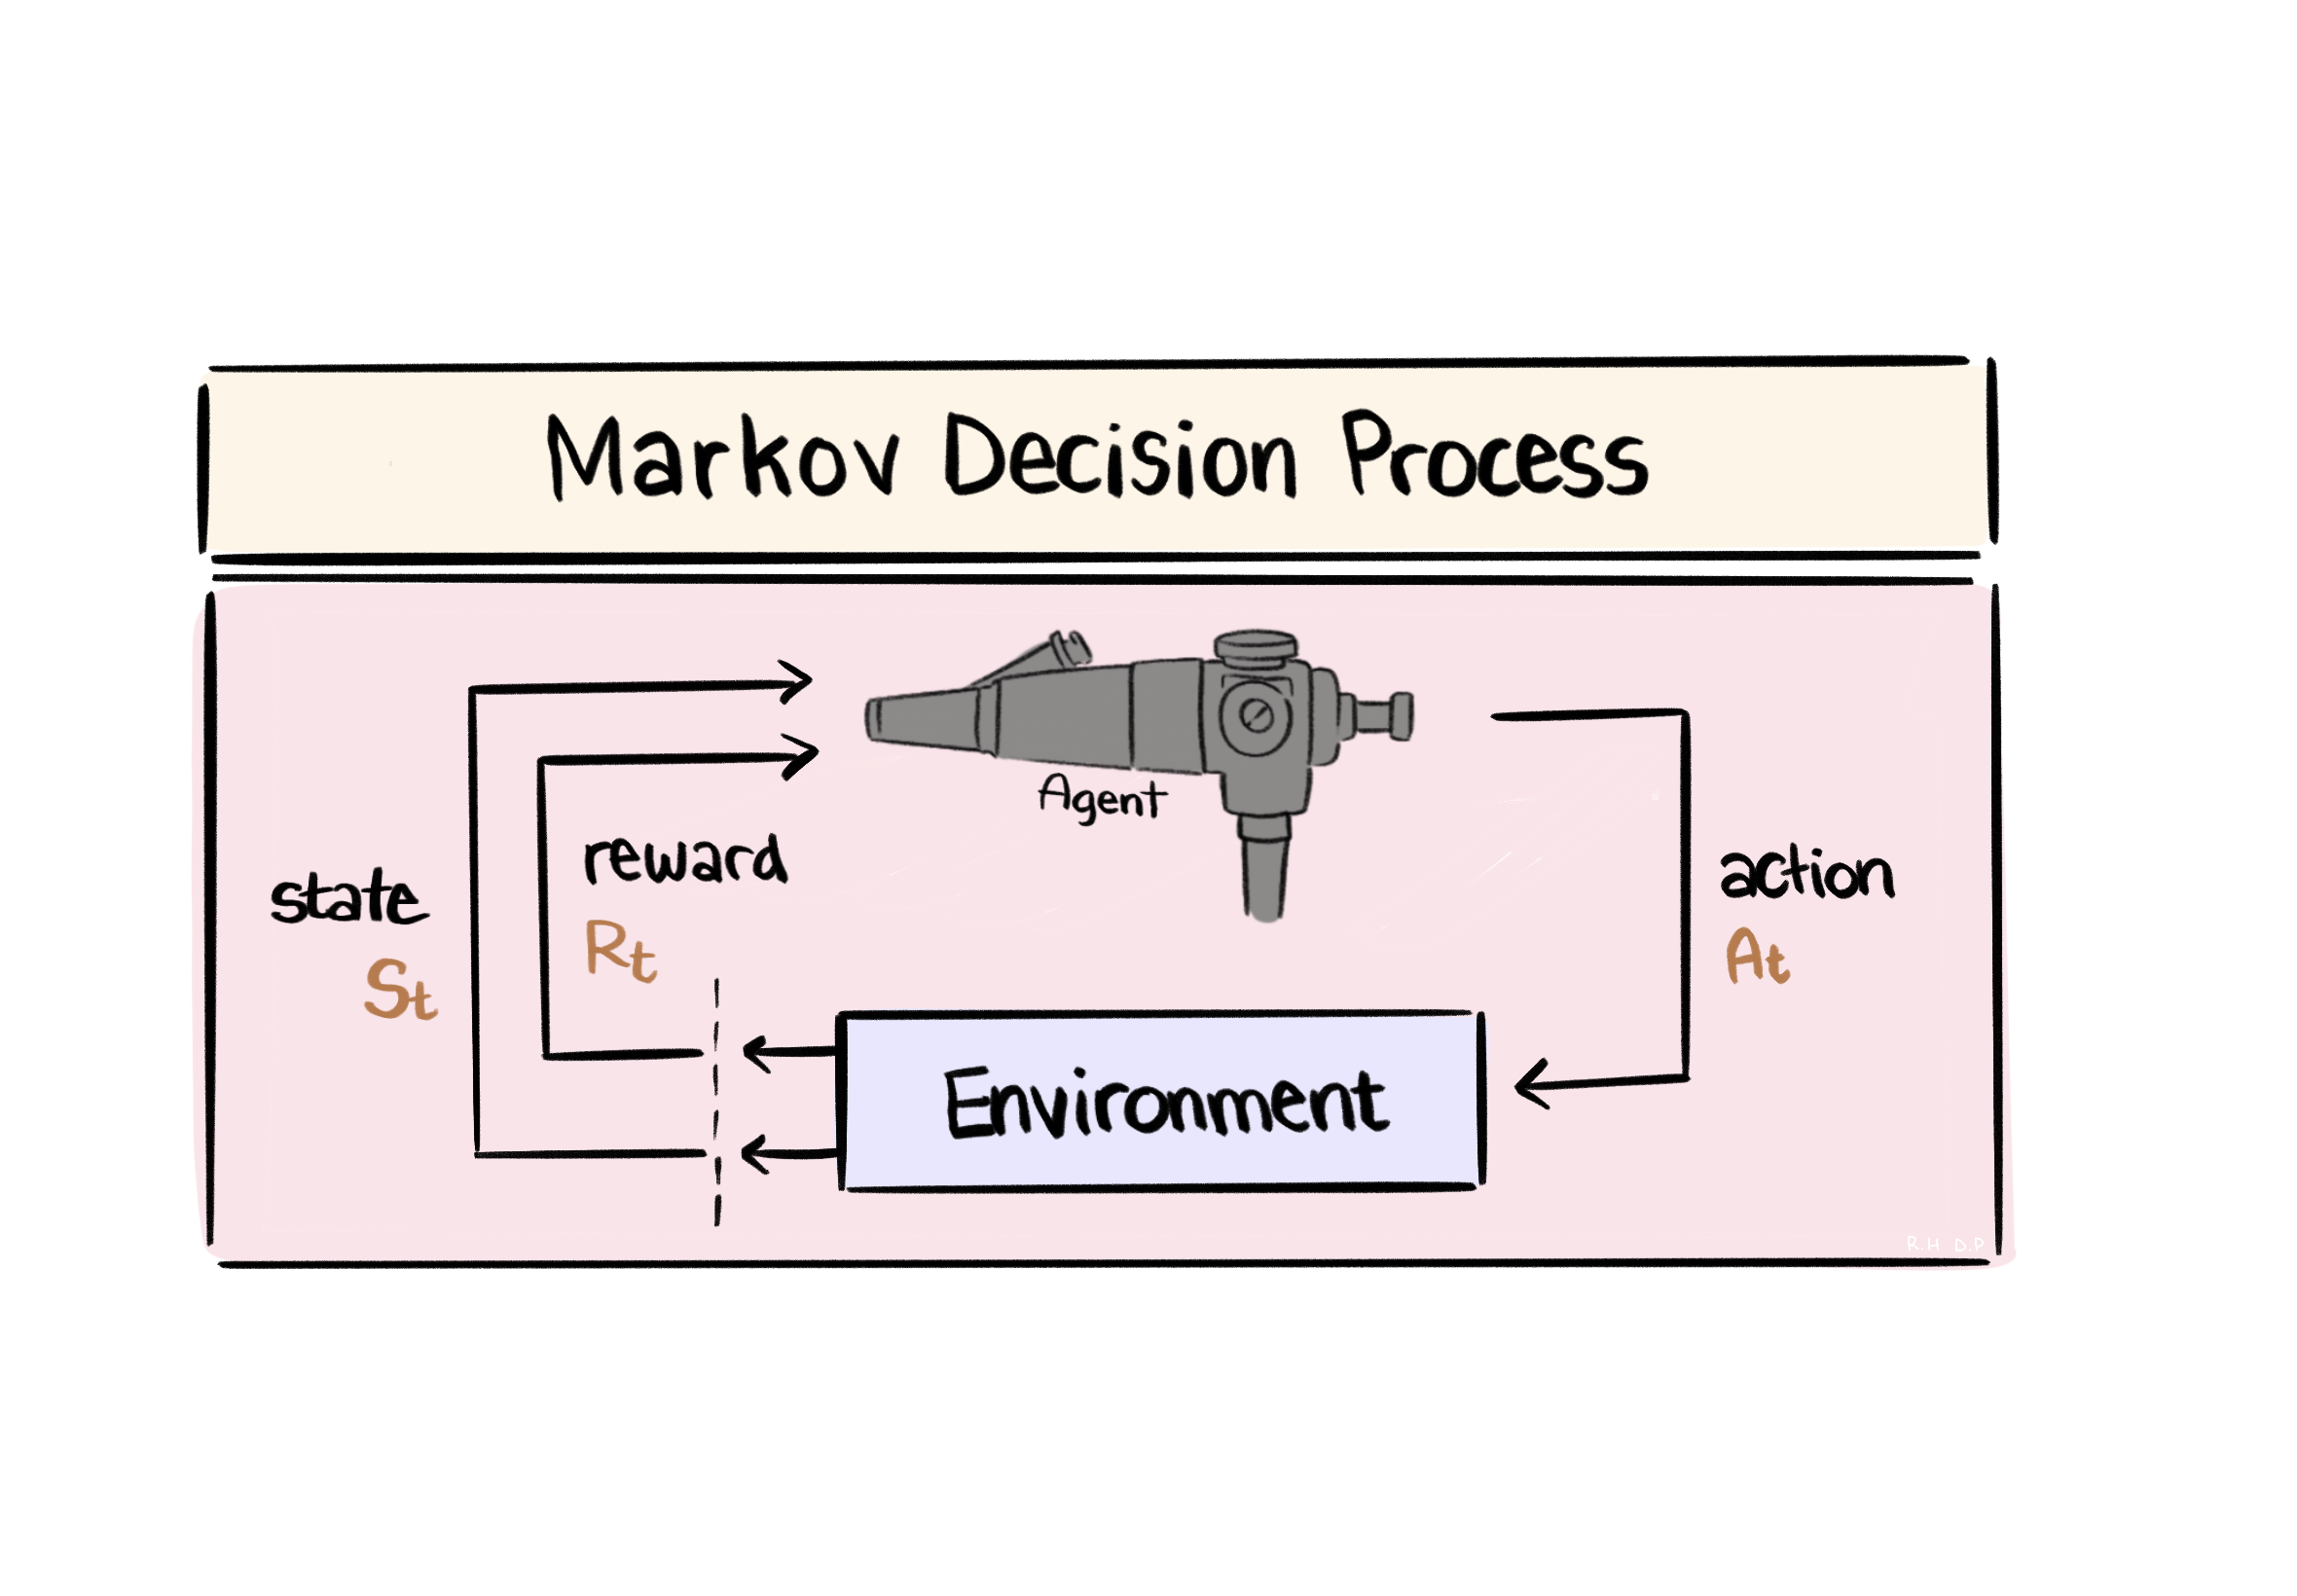
\includegraphics[width=0.8\linewidth,trim=0 6cm 0 6cm,clip]{assets/diagram-MDP.png}%
\caption{State transition and reward flow in an MDP.}
\label{fig:mdp_state_transition}
\end{figure}

\subsection{Value and Policy Methods}
There are two main ways to solve an RL problem. The first is \textbf{value-based learning}. Here the agent learns how good each action is. The second is \textbf{policy-based learning}. Here the agent learns the action rule directly.

Value methods such as Q-learning are simple and useful, especially when the action space is small. Policy methods are often better for continuous control, where the agent needs to steer smoothly instead of choosing from a short list of actions. That is why this work focuses on policy methods and actor-critic ideas, especially PPO \cite{schulman2017ppo}.

\begin{figure}[h]
\centering
\fbox{\parbox[b][3.4cm][c]{0.9\linewidth}{\centering Placeholder: value-based vs policy-based RL comparison}} 
\caption{Two main RL families: value-based and policy-based (placeholder).}
\label{fig:rl_taxonomy}
\end{figure}

\subsection{Why PPO Fits This Work}
PPO is popular because it keeps training stable. It updates the policy in small steps instead of making one big jump. That is helpful when the agent works in a noisy visual setting, where a big update could make the behaviour worse very quickly.

In simple terms, PPO tries to improve the agent without letting it become too adventurous at once. That is a good match for endoscopy, where we want progress, but not chaos. The policy should learn smooth and reliable behaviour, not dramatic surprises.

\begin{figure}[h]
\centering
\fbox{\parbox[b][3.6cm][c]{0.9\linewidth}{\centering Placeholder: PPO training loop with policy, critic, and clipped update}}
\caption{PPO training loop and clipped policy update (placeholder).}
\label{fig:ppo_loop}
\end{figure}

\subsection{Reward Design and Safety}
In a medical setting, reward design is a big deal. A bad reward can lead to odd behaviour. The agent may chase the score instead of the real goal. So rewards should be simple, clear, and tied to safe actions.

Useful ideas include:
\begin{itemize}
	\item \textbf{Reward shaping:} give small feedback during the task, not only at the end.
	\item \textbf{Penalties:} reduce reward for unsafe moves or bad tool contact.
	\item \textbf{Human review:} let clinicians check whether the behaviour looks sensible.
	\item \textbf{Simulation first:} train in a virtual setting before any real-world test.
\end{itemize}

\begin{figure}[h]
\centering
\fbox{\parbox[b][3.2cm][c]{0.9\linewidth}{\centering Placeholder: reward design diagram showing progress reward and safety penalties}}
\caption{Example reward design for safe RL (placeholder).}
\label{fig:reward_design}
\end{figure}

\subsection{Exploration}
RL also needs exploration. The agent must try new things to improve, but it should not take wild risks all the time. A small amount of exploration is good; too much is noisy; too little makes learning slow.

In practice, we often use controlled exploration such as action noise or epsilon-style randomness. In safety-critical tasks, simulation is the place to explore more freely, because the agent can fail there without harming a patient.

\subsection{RL in Endoscopy}
RL is useful in endoscopy because the task is sequential and visual. The agent may need to move the scope, keep the target in view, and decide when to act. This is not a single-frame problem. It is more like a short story: one move changes the next scene, and the next scene changes the next decision.

Recent work in surgical and medical robotics shows the same pattern: learning in simulation, safety constraints, and sim-to-real transfer are the big challenges \cite{qian2023arxiv,pore2022iros,corsi2023arxiv,ou2023lra,surrol2021arxiv}.

\begin{table}[h]
\centering
\caption{Simple view of RL methods used in this chapter}
\begin{tabular}{|l|l|l|}
\hline
\textbf{Method} & \textbf{Main idea} & \textbf{Why it helps} \\ \hline
Q-learning & Learn action values & Simple for discrete actions \\ \hline
Actor-critic & Policy + critic & More stable learning \\ \hline
PPO & Safe policy updates & Good for continuous control \\ \hline
\end{tabular}
\label{tab:rl_methods_short}
\end{table}

\subsection{Summary}
RL gives us a clean way to teach an agent step by step. In this project, the agent must learn safe and useful actions for navigation and extraction, so we focus on policy-based methods, especially PPO. The next chapter explains PPO in more detail.


\clearpage
\section{Convolutional Neural Networks (CNN) for Endoscopic Vision}
\label{sec:cnn}

\subsection*{Introduction}
Convolutional Neural Networks (\textbf{CNNs}) are deep learning models designed to process grid-like data, especially images. Their key idea is to learn local visual patterns through convolutional filters and to reuse the same weights across the input space. This gives CNNs strong performance on tasks that involve spatial structure.

CNNs are one of the most important ideas in modern computer vision, and they are used a lot in image classification, feature extraction, segmentation, and medical imaging \cite{lecun1998cnn,goodfellow2016deep,litjens2017dlSurvey}.

Some of the biggest milestones in CNNs are \textbf{AlexNet}, \textbf{ResNet}, and \textbf{U-Net} \cite{krizhevsky2012alexnet,he2016resnet,ronneberger2015unet}.

\subsection{Core Building Blocks}
The typical CNN pipeline consists of convolution layers, activation functions, pooling layers, and one or more fully connected layers at the end. Each part serves a distinct purpose:

\begin{itemize}
\item \textbf{Convolution:} Extracts local features such as edges, textures, and shapes.
\item \textbf{Activation:} Adds non-linearity, commonly using ReLU.
\item \textbf{Pooling:} Reduces spatial size and improves robustness to small translations.
\item \textbf{Dense Layers:} Combine extracted features to produce final predictions.
\end{itemize}

\begin{table}[h]
\centering
\caption{Main components of a CNN}
\begin{tabular}{|l|l|l|}
\hline
\textbf{Component} & \textbf{Function} & \textbf{Effect} \\ \hline
Convolution layer & Feature extraction & Detects local patterns \\ \hline
ReLU activation & Non-linearity & Improves expressive power \\ \hline
Pooling layer & Downsampling & Reduces feature map size \\ \hline
Flatten layer & Reshaping & Connects to dense layers \\ \hline
Fully connected layer & Classification/regression & Produces final output \\ \hline
\end{tabular}
\label{tab:cnn_components}
\end{table}

\begin{figure}[h]
\centering
\fbox{\parbox[b][3.5cm][c]{0.9\linewidth}{\centering Placeholder: CNN architecture diagram (conv → pool → FC)}}
\caption{CNN architecture (placeholder).}
\label{fig:cnn_arch}
\end{figure}

\subsection{Why CNNs Work Well for Vision Tasks}
CNNs are effective because they exploit two key properties of images: local spatial correlation and translation consistency. Instead of connecting every input pixel to every hidden unit, CNNs focus on local receptive fields and share filters across the image. This reduces the number of parameters and improves generalization.

\begin{table}[h]
\centering
\caption{Typical CNN applications}
\begin{tabular}{|l|l|l|}
\hline
\textbf{Application} & \textbf{Input Type} & \textbf{Output} \\ \hline
Image encoding & Natural images & Visual features \\ \hline
Appearance modelling & Images or video frames & Local descriptors \\ \hline
Segmentation & Medical or scene images & Pixel-wise labels \\ \hline
OCR and document analysis & Scanned pages & Text or layout features \\ \hline
Industrial inspection & Product images & Defect features \\ \hline
\end{tabular}
\label{tab:cnn_applications}
\end{table}

\subsection{CNNs for Navigation and Extraction}
In this work, CNNs are used as visual encoders for two kinds of image input: colon wall
images and target polyp images. The goal is not to build a polyp detector. Instead, the
CNN helps the agent understand the scene, keep the colon in view, and support the next
action during navigation or extraction.

For navigation, CNN features can help the agent recognise folds, bends, lighting changes,
and the current camera view. For extraction, they can help describe the polyp shape,
position, and nearby tissue so the agent can place tools more carefully. In both cases,
the CNN acts as a perception front-end for the decision policy.

The basic idea is simple: image input goes in, compact visual features come out, and the
policy uses those features to choose the next action. That is the bridge between vision
and control in this project.

Evaluation typically uses metrics that capture both feature quality and downstream
usefulness:
\begin{figure}[h]
\centering
\fbox{\parbox[b][3.5cm][c]{0.9\linewidth}{\centering Placeholder: colon wall and polyp image input for the agent}}
\caption{Example colon wall and polyp image input for the agent (placeholder).}
\label{fig:endoscopic_example}
\end{figure}

\begin{table}[h]
\centering
\caption{Common evaluation metrics for endoscopic visual encoders}
\begin{tabular}{|l|l|l|}
\hline
\textbf{Task} & \textbf{Metric} & \textbf{What It Measures} \\ \hline
Visual encoding & Representation quality & How well features summarize the image \\ \hline
Navigation support & Stability / latency & Real-time usefulness for control \\ \hline
Extraction support & Robustness & How well features work under lighting and motion changes \\ \hline
Deployment & Latency / stability & Real-time usability, reduced flicker \\ \hline
\end{tabular}
\label{tab:endoscopy_metrics}
\end{table}

Practical constraints include strong appearance variability, specular highlights,
occlusions, motion blur, and changes in colon wall texture. These factors motivate
robust training practices such as data augmentation and careful validation across
different acquisition conditions.

\subsection{Limitations}
Despite their success, CNNs have limitations:

\begin{itemize}
\item They require large annotated datasets for strong performance.
\item They are less natural for long-range temporal dependencies than sequence models.
\item Very deep networks can be expensive to train and deploy.
\end{itemize}

\subsection{Summary}
CNNs are still a foundational architecture for visual recognition tasks and are
especially useful for endoscopic perception modules. In this project, they turn images
of the colon wall and the target polyp into useful features for the agent. Those features
are then fed into higher-level decision systems that handle navigation and extraction.
\section{Temporal Modeling with Long Short-Term Memory Networks (LSTM)}
\label{sec:lstm}

\subsection*{Introduction}
Long Short-Term Memory (\textbf{LSTM}) networks are a type of recurrent neural network designed to model sequential data while reducing the vanishing gradient problem that affects standard RNNs \cite{hochreiter1997lstm}. They are especially useful when the current output depends on information from earlier time steps.

LSTMs are widely used in natural language processing, time-series prediction, speech
processing, and any other task where sequence context matters.

\subsection{Internal Mechanism}
An LSTM cell controls information flow using gates that decide what to remember, what to forget, and what to output. The cell state acts as a memory path that can carry information across many time steps.

The main gates are pretty easy to remember:

\begin{itemize}
\item \textbf{Forget gate:} Decides which parts of the previous memory to keep.
\item \textbf{Input gate:} Controls which new information should be stored.
\item \textbf{Output gate:} Determines the visible hidden state at the current step.
\end{itemize}

\begin{table}[h]
\centering
\caption{LSTM gates and their roles}
\begin{tabular}{|l|l|l|}
\hline
\textbf{Gate} & \textbf{Role} & \textbf{Purpose} \\ \hline
Forget gate & Filters old information & Removes irrelevant memory \\ \hline
Input gate & Controls new information & Stores useful context \\ \hline
Output gate & Exposes hidden state & Produces current output \\ \hline
\end{tabular}
\label{tab:lstm_gates}
\end{table}

\begin{figure}[h]
\centering
\fbox{\parbox[b][3.2cm][c]{0.9\linewidth}{\centering Placeholder: LSTM cell diagram (input, forget, output gates)}}
\caption{LSTM cell (placeholder).}
\label{fig:lstm_cell}
\end{figure}

\subsection{Sequence Modeling Strengths}
\begin{flushleft}
Compared with standard feed-forward networks, LSTMs are much better for ordered data
because they preserve temporal context. Compared with simple RNNs, they are also more
stable during training and can capture longer dependencies.

\begin{table}[h]
\centering
\caption{Common LSTM application areas}
\begin{tabular}{|l|l|l|}
\hline
\textbf{Domain} & \textbf{Task} & \textbf{Benefit} \\ \hline
Text processing & Language modeling & Context awareness \\ \hline
Speech analysis & Signal interpretation & Temporal continuity \\ \hline
Time series & Forecasting & Sequential dependency handling \\ \hline
Healthcare & Patient monitoring & Event trend modeling \\ \hline
Anomaly detection & Sensor streams & Pattern deviation detection \\ \hline
\end{tabular}
\label{tab:lstm_applications}
\end{table}

\end{flushleft}

\subsection{Relevance to Endoscopic Video}
\begin{flushleft}
Endoscopy produces video streams where the useful information often depends on what
happened a moment ago: lesions may be partially visible, the camera viewpoint changes
quickly, and short-term tracking can reduce flickering predictions. In this setting,
LSTMs can help to:

\begin{itemize}
	\item smooth frame-level predictions by integrating recent history;
	\item model tool or lesion motion as a sequence;
	\item support recognition of procedural phases (high-level temporal structure).
\end{itemize}

In many modern pipelines, attention-based models may replace recurrent networks for
longer contexts, but LSTMs are still a useful and lightweight baseline for temporal
aggregation.
\end{flushleft}

\subsection{Limitations}
\begin{flushleft}
LSTMs are powerful, but they can be slower to train than simpler networks and may still
struggle with very long sequences. In many recent applications, they are being
complemented or replaced by attention-based models, but they remain very important for
understanding recurrent sequence modeling.
\end{flushleft}

\subsection{Summary}
\begin{flushleft}
LSTMs provide a clean way to learn from ordered data by keeping a memory state across
time. They also form an important bridge between classical recurrent networks and newer
sequence modeling approaches.
\end{flushleft}
\clearpage
\section{Proximal Policy Optimization (PPO)}
\label{sec:ppo}

\subsection{Challenges of Large Policy Updates}

In deep reinforcement learning, the agent improves by updating its policy after collecting experience from the environment. But there is a tricky problem: if the update is too big, the policy can change so much that it starts making terrible decisions. This is a bit like a student who learns one good trick and then overuses it everywhere, even where it does not apply. The agent's performance can collapse overnight.

\begin{figure}[H]
\centering
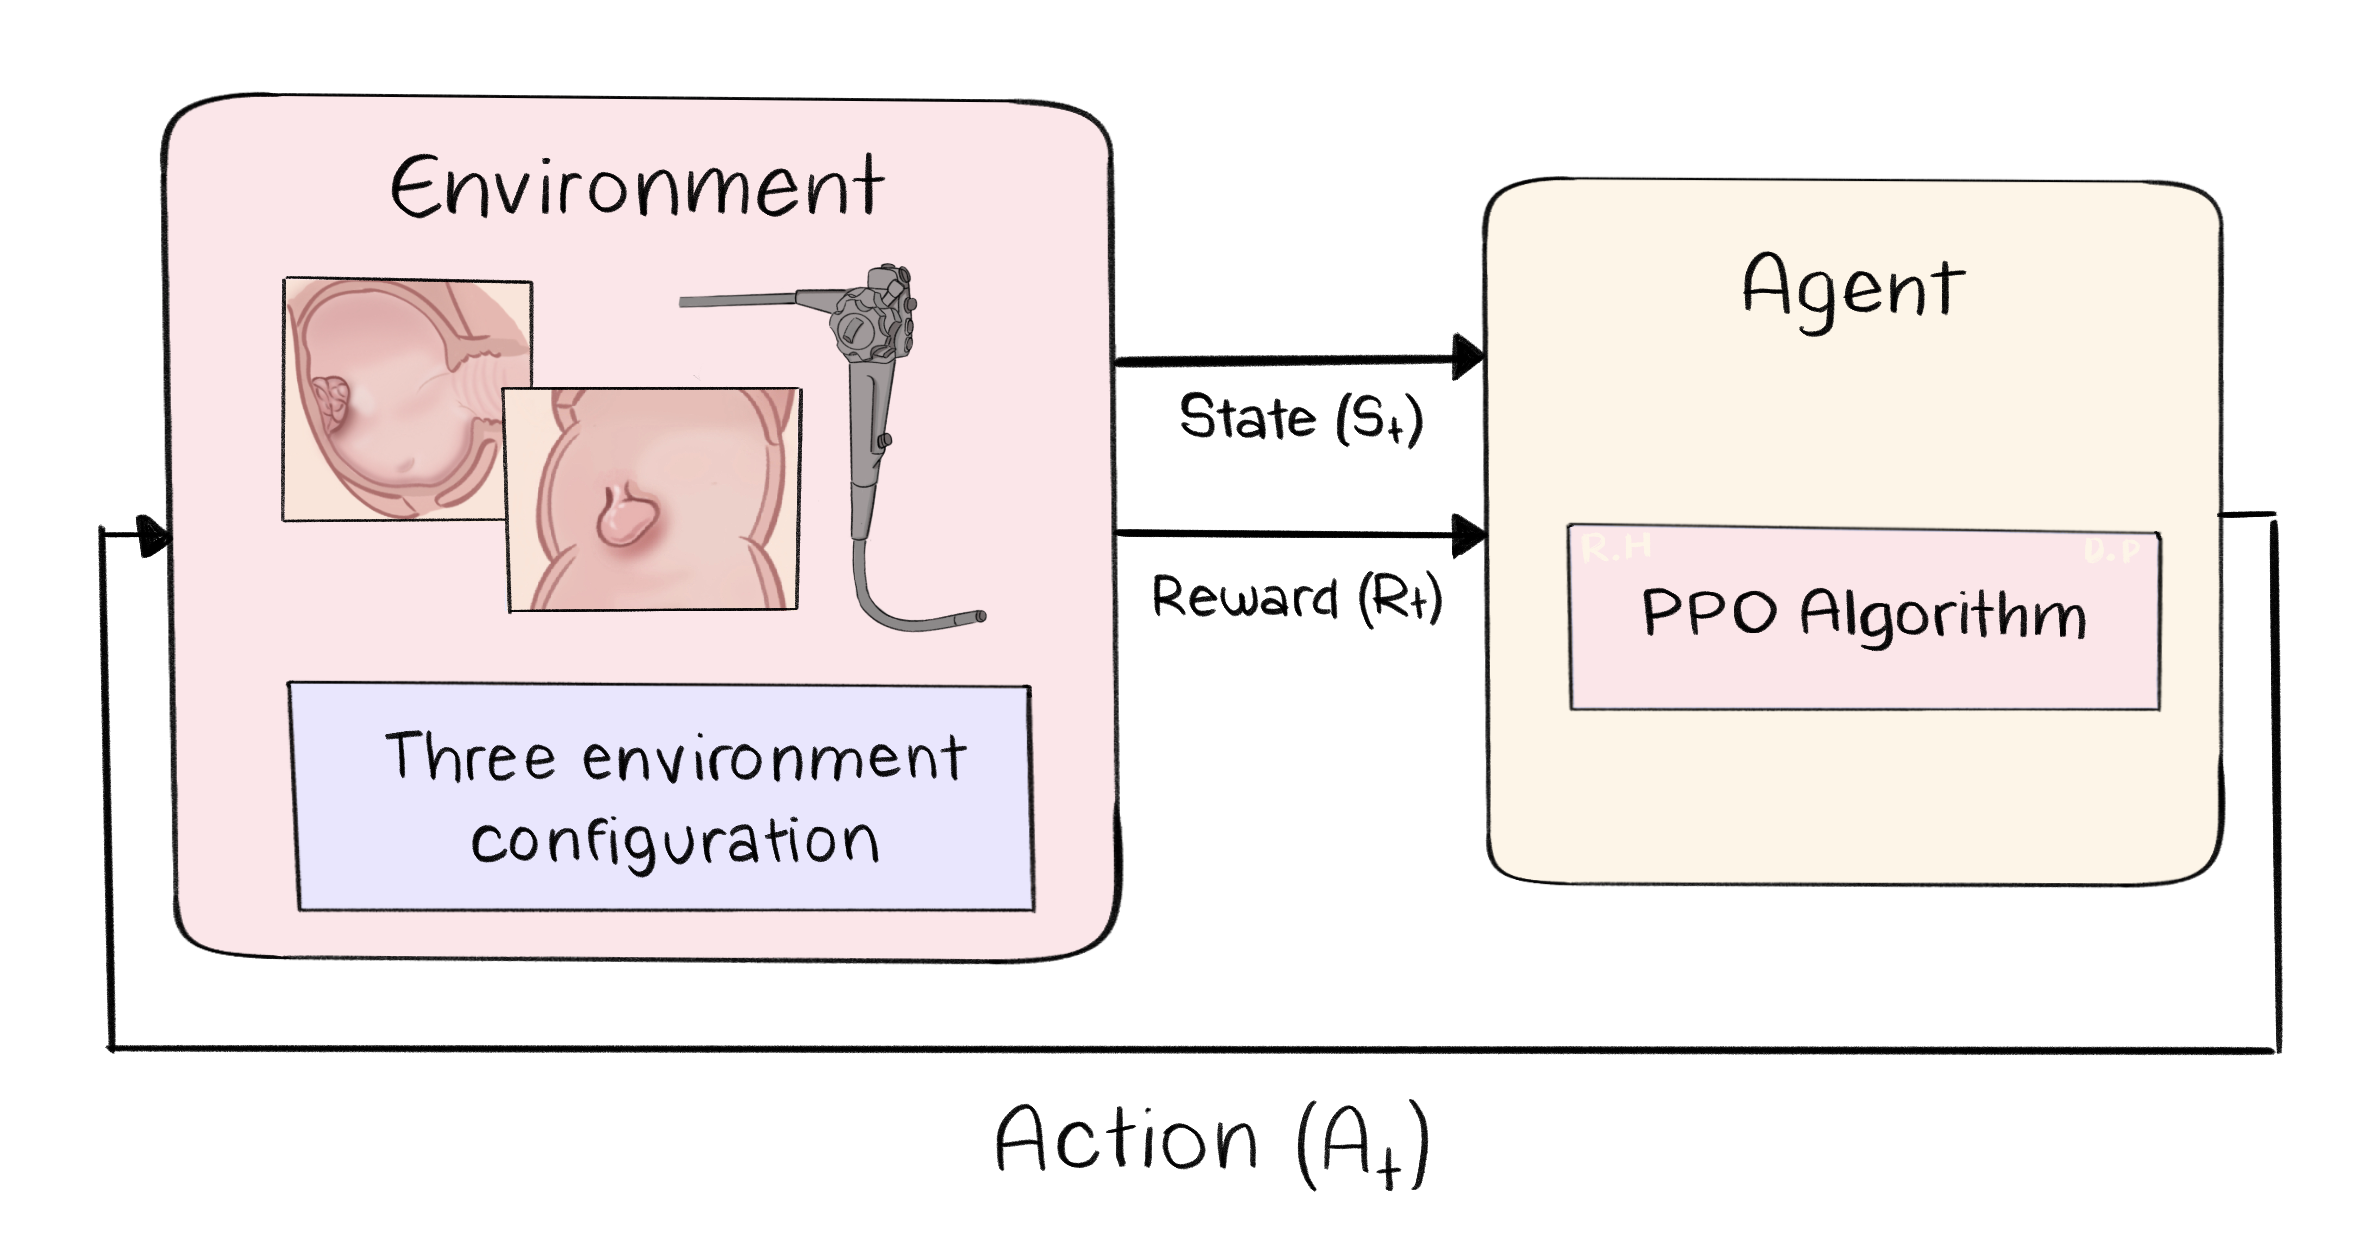
\includegraphics[width=0.8\linewidth]{assets/diagram-ppo-generic.png}
\caption{PPO Generic Architecture}
\label{fig:ppo_generic}
\end{figure}

Early policy gradient methods like \textbf{REINFORCE} suffered from this exact issue \cite{williams1992reinforce}. They had high variance, meaning the learning signal was very noisy, and a single bad update could undo hours of training. To fix this, researchers came up with \textbf{Trust Region Policy Optimization} (TRPO), which adds a mathematical constraint to make sure each update stays small and safe \cite{schulman2015trpo}. The idea is to keep the new policy ``close'' to the old one, measured by a quantity called the \textbf{KL divergence}.

TRPO works well in theory, but it is complicated to implement and slow to run because it needs second-order optimisation (computing the Hessian matrix). That is where PPO comes in.

\subsection{Stabilizing Learning with PPO Clipping}

\textbf{Proximal Policy Optimization} (PPO) was introduced by Schulman et al. at OpenAI in 2017, and it quickly became one of the most popular Deep RL algorithms in the world \cite{schulman2017ppo}. The reason is simple: PPO gives you most of the stability benefits of TRPO, but with a much simpler implementation.

The core idea is to use a \textbf{clipped objective function}. Instead of adding a hard mathematical constraint like TRPO does, PPO clips the policy update so it cannot go too far. Here is how it works:

The algorithm computes a \textbf{probability ratio} $r_t(\theta) = \frac{\pi_\theta(a_t|s_t)}{\pi_{\theta_\text{old}}(a_t|s_t)}$, which tells us how much the new policy differs from the old one for a given action. If this ratio stays close to 1, the update is small. If it gets too far from 1, PPO clips it back. The objective function is:

$$L^{\text{CLIP}}(\theta) = \mathbb{E}\left[\min\left(r_t(\theta) \hat{A}_t,\; \text{clip}(r_t(\theta),\; 1-\epsilon,\; 1+\epsilon)\; \hat{A}_t\right)\right]$$

where $\hat{A}_t$ is the \textbf{advantage estimate} (how much better this action was compared to the average) and $\epsilon$ is the clipping range, usually set to \textbf{0.1 or 0.2}. The $\min$ function makes sure that the agent cannot benefit from making the ratio too large in either direction.

In simple terms: PPO says ``improve, but do not go crazy.'' If the update would change the policy too much, PPO automatically limits it. This is what makes training so stable compared to older methods.


\subsection{The Actor-Critic Setup}

PPO uses an \textbf{actor-critic} architecture, which means it has two components working together:

\begin{itemize}
\item The \textbf{Actor} is the policy network. It takes the current state as input and outputs a probability distribution over possible actions. This is the part that actually decides what to do.
\item The \textbf{Critic} is the value network. It takes the same state as input and outputs a single number: an estimate of how much total reward the agent can expect from this state onwards. This is used to compute the advantage $\hat{A}_t$.
\end{itemize}

The advantage is calculated using \textbf{Generalized Advantage Estimation} (GAE), which combines multiple steps of rewards and value estimates to get a signal that is both low-variance and reasonably accurate \cite{schulman2016gae}:

$$\hat{A}_t = \sum_{l=0}^{T-t-1} (\gamma \lambda)^l \left(r_{t+l} + \gamma V_\phi(s_{t+l+1}) - V_\phi(s_{t+l})\right)$$

In many implementations, including ours, the actor and critic share the same neural network backbone (the CNN and LSTM layers) and only split at the final output heads. This means the visual features learned by the CNN are used by both the policy and the value function, which is more efficient.

The training loop looks like this: the agent collects a batch of experience by interacting with the environment, then uses that batch to update both the actor and the critic over several passes (called \textbf{epochs}). After the update, it throws away the old data and collects a fresh batch. This makes PPO an \textbf{on-policy} algorithm, which means it always learns from data generated by its current policy.

\begin{table}[H]
\centering
\caption{Key PPO hyperparameters and their typical values}
\begin{tabular}{|L{5cm}C{4.5cm}R{5cm}|}
\hline
\textbf{Hyperparameter} & \textbf{Typical range} & \textbf{What it controls} \\ \hline
Clipping range ($\epsilon$) & 0.1 to 0.2 & How much the policy can change per update \\ \hline
Discount factor ($\gamma$) & 0.95 to 0.99 & How much the agent cares about future rewards \\ \hline
GAE lambda ($\lambda$) & 0.9 to 0.99 & Balance between bias and variance \\ \hline
Learning rate & $10^{-4}$ to $10^{-3}$ & Speed of gradient updates \\ \hline
Epochs per update & 3 to 10 & How many passes over each batch \\ \hline
Entropy coefficient & 0.0 to 0.01 & Encourages exploration \\ \hline
\end{tabular}
\label{tab:ppo_hyperparams}
\end{table}

\subsection{Suitability of PPO for the Simulation}

We chose PPO for this project for several practical reasons. First, it is \textbf{stable}. Endoscopy is a task with noisy visual input (reflections, motion blur, changing lighting), and PPO handles that noise well because it does not overreact to any single batch of data. Second, it is \textbf{simple to implement}. The clipped objective is just a few lines of code, and excellent open-source libraries like \textbf{Stable Baselines3} provide ready-to-use PPO implementations. Third, it works well with \textbf{continuous actions}, which is important because our agent needs to output smooth, precise movements rather than choosing from a small set of discrete options.

PPO has also proven itself in many related domains. It is used to train robotic arms in simulation \cite{schulman2017ppo}, to fine-tune large language models with human feedback (the famous RLHF pipeline), and to control agents in complex video games. In surgical robotics, several recent papers have used PPO as their main training algorithm with good results \cite{qian2023arxiv,pore2022iros}.

Finally, PPO pairs well with the rest of our architecture. The CNN extracts visual features, the LSTM adds temporal context, and PPO uses both to learn a policy that improves over time. The clipping mechanism makes sure that even when the simulation produces unexpected situations (a sudden camera movement, an unusual polyp position), the learning process does not break down.

In the Contributions chapter, we will show the exact PPO configuration we used, the reward curves during training, and how the agent's behaviour improved over time.


\section*{Conclusion}
\addcontentsline{toc}{section}{Conclusion}
The state of the art makes one thing pretty clear: reliable assistance in endoscopy
needs both strong \textbf{perception} and solid \textbf{decision-making}. Vision models have to deal with
different patients, devices, lighting conditions, bowel preparation, occlusions, and
motion artifacts. Decision policies also need to stay stable under uncertainty and behave
in a way that actually makes sense clinically.

Across the literature, the same challenges keep showing up: rare events are hard to
collect, annotations take time, models often fail to generalize across sites, and
evaluation needs to reflect \textbf{safety constraints}, not just accuracy. These gaps are the
reason this work focuses on controlled training, careful reward design, and task-level
metrics that capture both \textbf{performance} and \textbf{safety}.

	% Methods chapter content has been moved to Chapter: Contributions.
% The detailed Methods sections are now part of `chapters/200_contributions.tex`.
% This file is intentionally left blank to avoid creating a separate "Methods"
% chapter in the compiled document.

	\chapter{Contributions}
\label{chap:contributions}

\section*{Introduction}
This chapter explains what was actually built in the project. The main contribution is a
two-phase Unity simulation where reinforcement learning is used for endoscope
navigation and snare capture. I keep the wording simple here on purpose, because the
important part is the system itself, not fancy language.

The work is split into two parts:

\begin{itemize}
	\item Phase~1 learns how to steer the endoscope through a colon-like path while
	forward movement is scripted.
	\item Phase~2 learns how to control the snare and capture a predefined polyp object
	using discrete actions and reward shaping.
\end{itemize}

This setup helped keep the problem manageable. Instead of trying to solve everything at
once, the project separates navigation from capture, which makes training, debugging,
and evaluation much easier.

Another contribution is the way the environment is structured. The agents use only
camera input, the rewards are designed around safety and progress, and the capture task
uses layered gating so the policy cannot just rush into the target without learning the
right sequence.

Finally, the report and code documentation were written so the experiments can be
reproduced more easily. That includes the PPO configuration files, the network
structure, and the main Unity scripts used in each phase.
 

\section{Overview}
\addcontentsline{toc}{section}{Overview}
This section expands the description of the implemented two-phase reinforcement
learning system. The goal is to learn endoscope navigation and an associated
snare-capture behavior in a simulated Unity environment. Important clarification:
the system does \emph{not} perform polyp detection or classification. The agent
policies are vision-only and map tip-camera images to discrete control actions.

\section{System Architecture}
\addcontentsline{toc}{section}{System Architecture}
The environment is implemented in Unity with ML-Agents for training. Key components
include `EndoscopeController` (tip kinematics and collision handling),
`EndoscopeActionDriver` (action mapping), `EndoscopeBurstPusher` (scripted insertion
for Phase~1), `PolypCaptureZone` and `PolypContactSensor` (layered capture logic), and
`SnareSlideController`.

The work is split into two phases to simplify exploration and evaluation:
\begin{itemize}
	\item Phase~1: navigation (steering only, scripted forward push).
	\item Phase~2: snare capture (steering + snare extension/rotation/open-close).
\end{itemize}

\section{Observations and Actions}
\addcontentsline{toc}{section}{Observations and Actions}
Both agents use a single tip-mounted RGB camera rendered at 80$\times$80 pixels. No
external detectors or segmentation masks are provided to the agents; policies learn
directly from images.

Phase~1 action space: one discrete branch with five actions (none, right, down,
left, up) that produce steering inputs. Forward motion is scripted by
`EndoscopeBurstPusher`.

Phase~2 action space: four discrete branches controlling steering (5 actions), snare
slide (3 actions), snare rotation (3 actions), and open/close (3 actions).

\section{Reward Design and Safety}
\addcontentsline{toc}{section}{Reward Design and Safety}
Rewards are shaped to encourage progress while discouraging unsafe contacts. Phase~1
uses a small alive reward, a goal bonus on reaching a trigger, and collision
penalties. Phase~2 uses layered rewards via `PolypCaptureZone` (increasing rewards
for progressing through layers), extension progress bonuses, and contact-based
outcomes (goal sphere = success, large sphere = penalty, colon contact = failure).

The report documents the exact numeric coefficients used during experiments; these
are reproduced in the `config/` YAML files.

\section{Network Architectures and Training}
\addcontentsline{toc}{section}{Network Architectures and Training}
Policies are trained with Proximal Policy Optimization (PPO). The visual encoder is a
small convolutional network that produces a 256-dimensional embedding, followed by
two 256-unit MLP layers and an LSTM memory module (sequence length 64, memory size
128). Policy heads are multi-categorical to match discrete branches. Phase~2 may
use an auxiliary curiosity signal to aid exploration.

Training hyperparameters (batch sizes, buffers, learning rates, schedules) are
stored in `config/endoscope_nav_ppo.yaml` and `config/snare_capture_ppo.yaml`.

\section{Evaluation Protocol}
\addcontentsline{toc}{section}{Evaluation Protocol}
Evaluation uses deterministic checkpoints and fixed seeds. Reported metrics include
success rate, collision rate, time-to-success, and layer progression statistics.
For reproducibility, list the number of seeds, evaluation episode count, and the
policy selection heuristic (best validation checkpoint vs last checkpoint).

\section{Limitations}
\addcontentsline{toc}{section}{Limitations}
This simulation uses Unity rigid-body physics and simplified spherical polyps. The
environment is intended for algorithmic investigation and not for clinical claims.
Where appropriate, the discussion in Chapter~\ref{chap:state_of_the_art} cites the
clinical and perception literature to contextualize results.

\section{Reproducibility}
\addcontentsline{toc}{section}{Reproducibility}
To reproduce experiments install the ML-Agents Python trainers version used during
development and match the Unity editor version. Include `config/` files, the exact
checkpoint hashes, and scripts to run evaluation.

\section{Files of Interest}
\addcontentsline{toc}{section}{Files of Interest}
See `Assets/` for Unity scripts and `config/` for trainer settings. Trainer source
details referenced in the repository's `.venv` folder are helpful for exact network
semantics.

	\chapter{General Conclusion}
\label{chap:general_conclusion}

\section*{Conclusion}
\begin{flushleft}
This thesis explored the compelling intersection of \textbf{computer vision}, \textbf{deep reinforcement learning}, and \textbf{endoscopic surgery} to tackle one of the most technically demanding procedures in modern medicine: \textbf{colorectal polypectomy}. The human colon has an internal surface area of roughly 2,000\,cm\textsuperscript{2}. Navigating this extensive anatomical structure and accurately deploying a snare around a polyp extends far beyond a simple image classification task. It is a highly complex, sequential decision-making problem, as each localized movement fundamentally alters the visual observation space.

To solve this, we built a highly sophisticated, physics-driven \textbf{Unity simulation} to train vision-only agents. We split the procedure into two separate parts: \textbf{endoscope navigation} and \textbf{snare capture}. This decoupling significantly reduced the control complexity for the agent. The resulting policies demonstrated strong efficacy. In the first phase, our agent learned to safely steer the endoscope tip through those tortuous haustral folds, actively dodging collisions by reading real-time visual cues like \textbf{specular highlights} and dynamic shadows, achieving a robust \textbf{best score of 14.67} after 6.5 million steps. In the second phase, the agent mastered the highly precise task of looping a snare around a pedunculated polyp. This was facilitated by a carefully engineered \textbf{spatial reward system} and an \textbf{Intrinsic Curiosity Module (ICM)}. Both phases relied heavily on \textbf{Proximal Policy Optimization (PPO)} paired with \textbf{Convolutional Neural Networks (CNNs)} and \textbf{LSTM memory} to deliver remarkably safe and reliable policies.

Ultimately, the core contribution of this work is proving that we can build a software-first, structured foundation for \textbf{adaptive, semi-autonomous systems} that can assist doctors in highly dynamic operating environments. 
\end{flushleft}

\section{Limitations}

While we are confident in the results achieved in this project, there are naturally a few limitations to keep in mind. First, to ensure the simulation executes with high computational efficiency, we opted out of using true \textbf{soft-tissue deformation}. Instead, we modeled the environment using efficient \textbf{geometric sphere-proxies} rather than fully anatomical soft-body physics. Finally, taking this technology from the simulator to the clinic means bridging the \textbf{sim-to-real gap}. Given the timeframe of this thesis, we simply didn't have enough time or access to a physical endoscope to rigorously test our trained models in a real hospital setting.

\section{Future Work}

Looking ahead, there are several promising avenues to explore. For future work, it would be highly beneficial to integrate a high-end biomechanical engine like \textbf{SOFA (Simulation Open Framework Architecture)} to handle realistic tissue deformation. An additional enhancement would be the integration of a dedicated \textbf{object-detection AI} (like YOLO) to spot the polyps automatically. This would create a powerful \textbf{hybrid system} where the computer vision model provides target coordinates to the Deep RL agent. Bridging the sim-to-real gap with richer clinical datasets and eventually testing these intelligent policies on real-world \textbf{robotic endoscopy hardware} remains a long-term objective.

	
\backmatter
	\bibliographystyle{unsrtnat}
	\bibliography{chapters/998_bibliography}
	\chapter*{Acronyms}
\addcontentsline{toc}{chapter}{Acronyms}

\begin{acronym} 
	
	\acro{RL}{Reinforcement Learning}
	\acro{PPO}{Proximal Policy Optimization}
    
\end{acronym} 

\end{document}